\documentclass[aspectratio=169,11pt]{beamer}
\usepackage[T1]{fontenc}
\usepackage{tgheros}
\usepackage{amsmath,amssymb,booktabs,array,tikz}
\usetikzlibrary{arrows.meta,positioning,calc,fit}
\renewcommand{\familydefault}{\sfdefault}
\renewcommand{\ttdefault}{lmtt}
\definecolor{Navy}{HTML}{162D46}
\definecolor{Teal}{HTML}{007F82}
\definecolor{Amber}{HTML}{B46D14}
\definecolor{Ink}{HTML}{263C4C}
\definecolor{Muted}{HTML}{617585}
\definecolor{Pale}{HTML}{EAF4F4}
\definecolor{Line}{HTML}{CCD8DF}
\setbeamercolor{normal text}{fg=Ink,bg=white}
\setbeamercolor{frametitle}{fg=Navy}
\setbeamercolor{title}{fg=Navy}
\setbeamercolor{structure}{fg=Teal}
\setbeamercolor{alerted text}{fg=Teal}
\setbeamerfont{title}{size=\LARGE,series=\bfseries}
\setbeamerfont{frametitle}{size=\Large,series=\bfseries}
\setbeamertemplate{navigation symbols}{}
\setbeamertemplate{itemize items}[circle]
\setbeamersize{text margin left=8mm,text margin right=8mm}
\newcommand{\stagecontext}{Data and terminology}
\newcommand{\stage}[1]{\gdef\stagecontext{#1}}
\setbeamertemplate{footline}{\hspace{8mm}\color{Muted}\scriptsize Bad Blood V2 \quad \stagecontext\hfill\insertframenumber\,/\,\inserttotalframenumber\hspace{8mm}\vspace{2.5mm}}
\setlength{\emergencystretch}{1.5em}
\newcommand{\source}[1]{\vfill\par{\fontsize{7}{8}\selectfont\color{Muted}#1}}
\newcommand{\takeaway}[1]{\par\medskip{\color{Teal}\bfseries #1}\par}
\newcommand{\whose}[1]{\par{\small\color{Teal}\textbf{Whose data?} #1}\par\medskip}
\newcommand{\pair}{\textsc{PairSE}}
\newcommand{\smalltable}{\fontsize{9}{11}\selectfont\renewcommand{\arraystretch}{1.18}}
\newcommand{\metricnote}{\par\smallskip{\scriptsize Values are SBP / DBP. Bold marks the best endpoint in this table. Lower errors, Bias closer to zero, and higher coverage are better.}}
\newcolumntype{P}[1]{>{\raggedright\arraybackslash}p{#1}}
\tikzset{>=Stealth, box/.style={draw=Line,fill=white,rounded corners=1.5pt,align=center,minimum height=9mm,inner sep=4pt,font=\small}, accent/.style={box,draw=Teal,fill=Pale}, conn/.style={->,thick,draw=Muted}, tinybox/.style={box,font=\scriptsize,inner sep=3pt}}
\hypersetup{pdftitle={Bad Blood V2: Models, Training, and Personalization},pdfauthor={Jingyi Guo},colorlinks=true,urlcolor=Teal,linkcolor=Navy}
\title{Blood Pressure Models,\ Training, and Personalization}
\subtitle{From many people's recordings to one person's model}
\author{\texorpdfstring{Jingyi Guo\\\small Bad Blood Project, University of Notre Dame}{Jingyi Guo, University of Notre Dame}}
\date{V2 results snapshot: October 15, 2026}
\begin{document}

\begin{frame}[plain]
\vspace{8mm}
{\color{Teal}\large BAD BLOOD V2}\par\vspace{4mm}
{\color{Navy}\LARGE\bfseries Blood Pressure Models,\\[2mm]Training, and Personalization}\par
\vspace{5mm}{\large From many people's recordings to one person's model}\par
\vspace{9mm}Jingyi Guo\\Bad Blood Project, University of Notre Dame\par
\vspace{4mm}{\small October 15, 2026}
\end{frame}

\begin{frame}{What the model predicts}
\textbf{Blood pressure (BP)} has two familiar numbers, such as 120/80.
\par\medskip
\begin{itemize}\setlength\itemsep{4mm}
\item \textbf{Systolic blood pressure (SBP)} is the higher pressure during a heartbeat.
\item \textbf{Diastolic blood pressure (DBP)} is the lower pressure between beats.
\item \textbf{mmHg} means millimeters of mercury, the pressure unit.
\end{itemize}
\par\medskip
Our model reads a \textbf{10-second segment}: ten seconds of signals from \textbf{one person}.
\takeaway{The output is two numbers for that segment: estimated SBP and DBP.}
\source{[7] The released models estimate segment-level pressure. A segment is also called a window.}
\end{frame}

\begin{frame}{PulseDB contains three waveforms and pressure labels}
\whose{Hospital participants in the public dataset. Each segment belongs to one person.}
\smalltable
\begin{tabular}{P{2.0cm}P{4.4cm}P{6.0cm}}\toprule
Field & Full name & What it records\\\midrule
ECG & Electrocardiogram & Heart electrical activity over time\\[2mm]
PPG & Photoplethysmogram & Optical changes related to blood volume over time\\[2mm]
ABP & Arterial blood pressure & Pressure inside an artery over time\\[2mm]
SBP, DBP & Systolic, diastolic blood pressure & Two scalar labels summarizing each segment\\\bottomrule
\end{tabular}
\takeaway{A waveform is a sequence of samples. A scalar label is one number.}
\source{[1] PulseDB includes recorded waveforms as well as derived labels. Its files also contain participant identifiers and other metadata.}
\end{frame}

\begin{frame}{Where ABP comes from, and how it gives the labels}
\whose{The same hospital participant and recording interval as the ECG and PPG.}
\begin{center}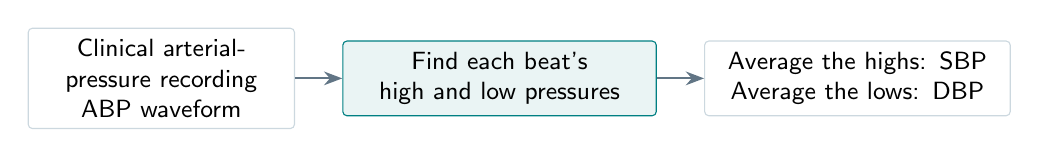
\begin{tikzpicture}
\node[box,text width=3.1cm] (a) {Clinical arterial-pressure recording\\ABP waveform};
\node[accent,right=6mm of a,text width=3.7cm] (b) {Find each beat's\\high and low pressures};
\node[box,right=6mm of b,text width=3.6cm] (c) {Average the highs: SBP\\Average the lows: DBP};
\draw[conn](a)--(b);\draw[conn](b)--(c);
\end{tikzpicture}\end{center}
\begin{itemize}\setlength\itemsep{3mm}
\item PulseDB carries the ABP waveform from its clinical source recordings.
\item It derives each 10-second segment's labels from the beats in that segment.
\item Our training code reads those supplied SBP/DBP labels.
\end{itemize}
\takeaway{ABP is recorded source data. We do not reconstruct it by interpolating SBP/DBP.}
\source{[1] PulseDB, Sections 2.2, 2.4.3 and 2.5. The two released models predict scalar labels rather than an ABP waveform.}
\end{frame}

\begin{frame}{What PulseDB provides versus what our model uses}
\begin{center}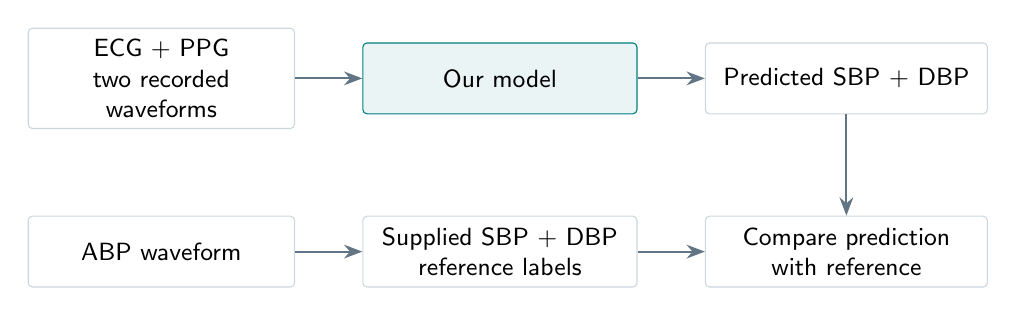
\begin{tikzpicture}[x=1cm,y=1cm]
\node[box,text width=3.1cm] (x) at(0,1.0){ECG + PPG\\two recorded waveforms};
\node[accent,text width=3.2cm] (m) at(4.3,1.0){Our model};
\node[box,text width=3.3cm] (p) at(8.7,1.0){Predicted SBP + DBP};
\node[box,text width=3.1cm] (a) at(0,-1.2){ABP waveform};
\node[box,text width=3.2cm] (y) at(4.3,-1.2){Supplied SBP + DBP\\reference labels};
\node[box,text width=3.3cm] (e) at(8.7,-1.2){Compare prediction\\with reference};
\draw[conn](x)--(m);\draw[conn](m)--(p);
\draw[conn](a)--(y);\draw[conn](y)--(e);\draw[conn](p)--(e);
\end{tikzpicture}\end{center}
\small The \textbf{PPG-only version} uses only the optical waveform. Neither version needs current ABP or current true BP as a prediction input.
\par\medskip
During training, the comparison updates weights. During testing, it only scores the saved model.
\source{[1] Label provenance. [7] Actual model inputs and scalar regression target. Later slides explain the extra earlier reference measurements used for personalization.}
\end{frame}

\begin{frame}{Public hospital data and our future student measurements}
\smalltable
\begin{tabular}{P{3.3cm}P{4.7cm}P{4.7cm}}\toprule
 & Current public-data experiments & Planned Notre Dame measurements\\\midrule
People & Hospital participants & Student volunteers\\[2mm]
Model signals & ECG and PPG recordings & ECG and PPG from our sensors\\[2mm]
Reference pressure & Labels from recorded ABP & Intermittent upper-arm cuff readings\\[2mm]
Continuous ABP & Present in PulseDB & Not collected by our proposed equipment\\[2mm]
Results in this deck & All reported results & No student results reported here\\\bottomrule
\end{tabular}
\takeaway{The current personal models also use public-data participants.}
\source{[1,7] Current experiment provenance. A student session with a few cuff readings supplies fewer reference labels than the dense public-data calibration studied here.}
\end{frame}

\begin{frame}{Whose data enters each of the four stages?}
\smalltable
\begin{tabular}{P{2.6cm}P{4.6cm}P{5.5cm}}\toprule
Stage & Whose recordings? & What happens to the model?\\\midrule
1. Group training & Many public-data participants & Learn a shared waveform-to-pressure model\\[2mm]
2. Group pair training & Same training group. Each pair comes from one person & Learn how pressure changes between two signal states\\[2mm]
3. Personal fitting & Only person P's early recordings and known pressure labels & Copy the shared model, then fit its last CNN block, SE and change head to P\\[2mm]
4. Personal testing & P's later signals, plus P's saved early references & Freeze weights. Predict P's later pressure and score it\\\bottomrule
\end{tabular}
\takeaway{Many people teach the starting model. One person's early data adapts their own copy.}
\source{[7] Stages 1 and 2 share source-training participants. Each target person gets an independent personal fit.}
\end{frame}

\begin{frame}{The people and the jobs of their data}

\whose{All groups come from the VitalDB-derived portion of PulseDB, not ND students.}
\smalltable\begin{tabular}{P{3.3cm}rrP{5.1cm}}\toprule
Group & People & Windows & Job\\\midrule
Group training & 1,085 & 390,600 & Learn shared weights\\
Group validation & 192 & 69,120 & Choose population checkpoints\\
Group main test & 141 & 56,400 & Score uncalibrated predictions\\
BP-range stress test & 116 & 666 & Different pressure range\\\midrule
Personal development & 30 & 8,882 & Each person's own early 80\%: train and select settings\\
Personal test & Same 30 & 2,211 & Each person's later 20\%: score only\\\bottomrule
\end{tabular}
\takeaway{Every target person selects settings using their own development data.}
\source{[7] A 10-second temporal guard removes boundary windows. Same 30 people across modes and seeds. These target records were previously examined; the current comparison is exploratory.}

\end{frame}

\begin{frame}{How the data is stored}
\begin{itemize}\setlength\itemsep{3mm}
\item \textbf{PulseDB} reorganizes recordings from VitalDB and MIMIC-III, another clinical database. We currently use its \textbf{VitalDB-derived portion}.
\item Original \textbf{MATLAB .mat files} contain waveforms, labels and participant information. Individual-record files also provide sample times in \texttt{T}.
\item Our prepared \texttt{waves.npy} is a NumPy array with shape $N\times2\times1250$.
\item Our \texttt{y.npy} has shape $N\times2$, holding SBP and DBP labels in the same window order.
\end{itemize}
\par\medskip
$N$ = number of windows. Each window contains \textbf{two signal channels} and \textbf{1,250 samples per channel}.
\takeaway{The training collection has many people. An individual row is still one person's window.}
\source{[1] Official file documentation. [7] shared/data.py. NumPy is the numerical-array library used by our Python pipeline. MIMIC-III: Medical Information Mart for Intensive Care III.}
\end{frame}

\begin{frame}{Model words used throughout this presentation}
\smalltable
\begin{tabular}{P{2.7cm}P{10.0cm}}\toprule
Term & Meaning here\\\midrule
CNN & Convolutional neural network. Learned filters scan the waveform.\\[2mm]
1D & One-dimensional. The filters move along the time axis.\\[2mm]
SE & Squeeze-and-Excitation. A small module weights learned feature traces.\\[2mm]
Encoder / backbone & The shared part that converts a waveform into 48 summary numbers.\\[2mm]
Head & The final part that converts features into a prediction.\\[2mm]
MLP & Multilayer perceptron. A stack of fully connected layers.\\[2mm]
PairSE & Our project's name for a paired-reference model built around CNN+SE.\\\bottomrule
\end{tabular}
\source{[2,3,7] PairSE is our implementation name. It is not the title of the published method that inspired it.}
\end{frame}

\begin{frame}{Training words used throughout this presentation}
\smalltable
\begin{tabular}{P{3.2cm}P{9.5cm}}\toprule
Term & Meaning here\\\midrule
Feature & A number computed from a window. It changes with the input.\\
Parameter / weight & A model value learned during training and saved afterward.\\
Batch & A set of windows used together for one weight update.\\
Step & One optimizer update of model weights.\\
Epoch & One pass through the group training windows.\\
Checkpoint & A saved version of model weights after training.\\
Seed & A number controlling random initialization and sampling.\\
Pretraining & Learning the shared starting model from a group.\\
Personal fitting & Updating a copy using one person's early labeled data.\\\bottomrule
\end{tabular}
\takeaway{Running the same model three times uses three seeds, not three new datasets.}
\source{[7] Our experiments use seeds 42, 43 and 44. All three use the same participant split.}
\end{frame}

\stage{One public-data participant: an example window}
\begin{frame}{One real person's ten seconds of input}
\textbf{Public test participant p000053\_1, row 0}
\begin{center}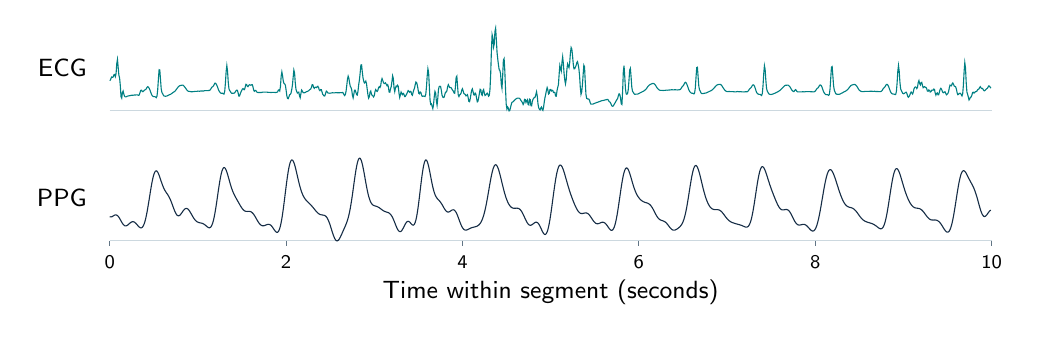
\begin{tikzpicture}[x=1.12cm,y=1cm]
\draw[draw=Line](0,0)--(10,0);\draw[draw=Line](0,1.65)--(10,1.65);
\begin{scope}[yshift=1.65cm]\draw[Teal,thin] plot coordinates {(0.00000,0.38406) (0.00800,0.39302) (0.01600,0.41638) (0.02400,0.43192) (0.03200,0.42606) (0.04000,0.43083) (0.04800,0.45898) (0.05600,0.46282) (0.06400,0.43568) (0.07200,0.47328) (0.08000,0.60016) (0.08800,0.65413) (0.09600,0.55275) (0.10400,0.45212) (0.11200,0.41863) (0.12000,0.32167) (0.12800,0.18228) (0.13600,0.16243) (0.14400,0.23361) (0.15200,0.25285) (0.16000,0.21437) (0.16800,0.18622) (0.17600,0.17898) (0.18400,0.17813) (0.19200,0.18202) (0.20000,0.18700) (0.20800,0.18924) (0.21600,0.19092) (0.22400,0.19319) (0.23200,0.19503) (0.24000,0.19677) (0.24800,0.19841) (0.25600,0.19873) (0.26400,0.19868) (0.27200,0.20016) (0.28000,0.20178) (0.28800,0.20214) (0.29600,0.20251) (0.30400,0.20325) (0.31200,0.20355) (0.32000,0.20144) (0.32800,0.19769) (0.33600,0.20560) (0.34400,0.23391) (0.35200,0.26112) (0.36000,0.26309) (0.36800,0.24970) (0.37600,0.24392) (0.38400,0.25095) (0.39200,0.26170) (0.40000,0.26750) (0.40800,0.27123) (0.41600,0.28318) (0.42400,0.30054) (0.43200,0.30773) (0.44000,0.30017) (0.44800,0.28574) (0.45600,0.26652) (0.46400,0.24077) (0.47200,0.21500) (0.48000,0.19753) (0.48800,0.18759) (0.49600,0.18158) (0.50400,0.18077) (0.51200,0.18183) (0.52000,0.17547) (0.52800,0.16815) (0.53600,0.18820) (0.54400,0.26624) (0.55200,0.40261) (0.56000,0.52323) (0.56800,0.52003) (0.57600,0.39710) (0.58400,0.27925) (0.59200,0.23378) (0.60000,0.21833) (0.60800,0.19980) (0.61600,0.18883) (0.62400,0.18720) (0.63200,0.18660) (0.64000,0.18695) (0.64800,0.18932) (0.65600,0.19294) (0.66400,0.19754) (0.67200,0.20214) (0.68000,0.20642) (0.68800,0.21070) (0.69600,0.21535) (0.70400,0.22152) (0.71200,0.22886) (0.72000,0.23525) (0.72800,0.24074) (0.73600,0.24729) (0.74400,0.25618) (0.75200,0.26756) (0.76000,0.27998) (0.76800,0.29194) (0.77600,0.30343) (0.78400,0.31299) (0.79200,0.31881) (0.80000,0.32210) (0.80800,0.32415) (0.81600,0.32554) (0.82400,0.32712) (0.83200,0.32608) (0.84000,0.31861) (0.84800,0.30719) (0.85600,0.29567) (0.86400,0.28311) (0.87200,0.26953) (0.88000,0.25836) (0.88800,0.25145) (0.89600,0.24835) (0.90400,0.24744) (0.91200,0.24619) (0.92000,0.24394) (0.92800,0.24261) (0.93600,0.24341) (0.94400,0.24477) (0.95200,0.24520) (0.96000,0.24633) (0.96800,0.24864) (0.97600,0.24876) (0.98400,0.24735) (0.99200,0.24924) (1.00000,0.25202) (1.00800,0.25071) (1.01600,0.24914) (1.02400,0.25094) (1.03200,0.25253) (1.04000,0.25260) (1.04800,0.25288) (1.05600,0.25274) (1.06400,0.25301) (1.07200,0.25538) (1.08000,0.25749) (1.08800,0.25741) (1.09600,0.25694) (1.10400,0.25732) (1.11200,0.25813) (1.12000,0.25877) (1.12800,0.25937) (1.13600,0.26310) (1.14400,0.27404) (1.15200,0.29010) (1.16000,0.30258) (1.16800,0.30796) (1.17600,0.31618) (1.18400,0.33470) (1.19200,0.35107) (1.20000,0.35134) (1.20800,0.33986) (1.21600,0.32299) (1.22400,0.29881) (1.23200,0.27228) (1.24000,0.25294) (1.24800,0.24002) (1.25600,0.22927) (1.26400,0.22369) (1.27200,0.22483) (1.28000,0.22433) (1.28800,0.21622) (1.29600,0.21362) (1.30400,0.24912) (1.31200,0.35325) (1.32000,0.49893) (1.32800,0.57597) (1.33600,0.50632) (1.34400,0.36616) (1.35200,0.28090) (1.36000,0.25998) (1.36800,0.24673) (1.37600,0.23032) (1.38400,0.22394) (1.39200,0.22448) (1.40000,0.22524) (1.40800,0.22428) (1.41600,0.22843) (1.42400,0.24255) (1.43200,0.25607) (1.44000,0.26388) (1.44800,0.26071) (1.45600,0.22875) (1.46400,0.18859) (1.47200,0.18755) (1.48000,0.21680) (1.48800,0.23927) (1.49600,0.25696) (1.50400,0.27763) (1.51200,0.28412) (1.52000,0.27174) (1.52800,0.26989) (1.53600,0.30148) (1.54400,0.33757) (1.55200,0.33643) (1.56000,0.31277) (1.56800,0.30824) (1.57600,0.32344) (1.58400,0.33243) (1.59200,0.32885) (1.60000,0.32608) (1.60800,0.33222) (1.61600,0.33329) (1.62400,0.30756) (1.63200,0.26688) (1.64000,0.24968) (1.64800,0.25853) (1.65600,0.25993) (1.66400,0.24593) (1.67200,0.23545) (1.68000,0.23360) (1.68800,0.23380) (1.69600,0.23427) (1.70400,0.23402) (1.71200,0.23274) (1.72000,0.23374) (1.72800,0.23674) (1.73600,0.23773) (1.74400,0.23764) (1.75200,0.23882) (1.76000,0.23918) (1.76800,0.23799) (1.77600,0.23761) (1.78400,0.23784) (1.79200,0.23698) (1.80000,0.23576) (1.80800,0.23535) (1.81600,0.23502) (1.82400,0.23407) (1.83200,0.23383) (1.84000,0.23500) (1.84800,0.23559) (1.85600,0.23546) (1.86400,0.23582) (1.87200,0.23434) (1.88000,0.23277) (1.88800,0.23543) (1.89600,0.23664) (1.90400,0.24226) (1.91200,0.26339) (1.92000,0.26764) (1.92800,0.25365) (1.93600,0.31089) (1.94400,0.43778) (1.95200,0.49487) (1.96000,0.44542) (1.96800,0.38037) (1.97600,0.34844) (1.98400,0.34256) (1.99200,0.32620) (2.00000,0.26538) (2.00800,0.19449) (2.01600,0.15813) (2.02400,0.15514) (2.03200,0.17915) (2.04000,0.20533) (2.04800,0.21054) (2.05600,0.22733) (2.06400,0.27072) (2.07200,0.32770) (2.08000,0.42513) (2.08800,0.51848) (2.09600,0.48442) (2.10400,0.35611) (2.11200,0.27487) (2.12000,0.24666) (2.12800,0.22679) (2.13600,0.23568) (2.14400,0.23873) (2.15200,0.19022) (2.16000,0.16701) (2.16800,0.22012) (2.17600,0.26541) (2.18400,0.25345) (2.19200,0.23314) (2.20000,0.23038) (2.20800,0.23075) (2.21600,0.23346) (2.22400,0.24018) (2.23200,0.24431) (2.24000,0.24657) (2.24800,0.25091) (2.25600,0.25730) (2.26400,0.26581) (2.27200,0.27284) (2.28000,0.27927) (2.28800,0.30182) (2.29600,0.33364) (2.30400,0.33144) (2.31200,0.29745) (2.32000,0.28604) (2.32800,0.30004) (2.33600,0.30141) (2.34400,0.29638) (2.35200,0.30519) (2.36000,0.31221) (2.36800,0.29659) (2.37600,0.26750) (2.38400,0.25708) (2.39200,0.27092) (2.40000,0.26940) (2.40800,0.23732) (2.41600,0.20979) (2.42400,0.19940) (2.43200,0.18865) (2.44000,0.19143) (2.44800,0.22391) (2.45600,0.25142) (2.46400,0.24528) (2.47200,0.22909) (2.48000,0.22532) (2.48800,0.22608) (2.49600,0.22477) (2.50400,0.22531) (2.51200,0.22802) (2.52000,0.22981) (2.52800,0.23010) (2.53600,0.22968) (2.54400,0.22911) (2.55200,0.22972) (2.56000,0.23171) (2.56800,0.23224) (2.57600,0.23055) (2.58400,0.23016) (2.59200,0.23112) (2.60000,0.23036) (2.60800,0.23038) (2.61600,0.23256) (2.62400,0.23171) (2.63200,0.23092) (2.64000,0.23439) (2.64800,0.22770) (2.65600,0.20624) (2.66400,0.19431) (2.67200,0.20805) (2.68000,0.24966) (2.68800,0.32305) (2.69600,0.40444) (2.70400,0.44227) (2.71200,0.41469) (2.72000,0.35434) (2.72800,0.31211) (2.73600,0.29828) (2.74400,0.26731) (2.75200,0.20004) (2.76000,0.16517) (2.76800,0.20978) (2.77600,0.26409) (2.78400,0.26331) (2.79200,0.23393) (2.80000,0.20553) (2.80800,0.20177) (2.81600,0.25807) (2.82400,0.33833) (2.83200,0.39811) (2.84000,0.48374) (2.84800,0.58290) (2.85600,0.58547) (2.86400,0.49662) (2.87200,0.42134) (2.88000,0.37990) (2.88800,0.35475) (2.89600,0.36394) (2.90400,0.37861) (2.91200,0.34398) (2.92000,0.27361) (2.92800,0.20491) (2.93600,0.16147) (2.94400,0.17922) (2.95200,0.23801) (2.96000,0.25196) (2.96800,0.21517) (2.97600,0.19505) (2.98400,0.19035) (2.99200,0.17720) (3.00000,0.19338) (3.00800,0.24410) (3.01600,0.27055) (3.02400,0.25832) (3.03200,0.24685) (3.04000,0.26009) (3.04800,0.29218) (3.05600,0.30884) (3.06400,0.29705) (3.07200,0.31520) (3.08000,0.37975) (3.08800,0.41027) (3.09600,0.38603) (3.10400,0.36117) (3.11200,0.34756) (3.12000,0.34682) (3.12800,0.35545) (3.13600,0.33792) (3.14400,0.32034) (3.15200,0.33234) (3.16000,0.30442) (3.16800,0.23966) (3.17600,0.23724) (3.18400,0.27887) (3.19200,0.30846) (3.20000,0.37126) (3.20800,0.44560) (3.21600,0.41171) (3.22400,0.29205) (3.23200,0.24519) (3.24000,0.29164) (3.24800,0.31470) (3.25600,0.30719) (3.26400,0.32598) (3.27200,0.31223) (3.28000,0.22635) (3.28800,0.17123) (3.29600,0.20502) (3.30400,0.23968) (3.31200,0.21978) (3.32000,0.20671) (3.32800,0.22264) (3.33600,0.21214) (3.34400,0.18201) (3.35200,0.18214) (3.36000,0.20048) (3.36800,0.21459) (3.37600,0.23738) (3.38400,0.25792) (3.39200,0.24983) (3.40000,0.23716) (3.40800,0.24855) (3.41600,0.24574) (3.42400,0.20865) (3.43200,0.19836) (3.44000,0.23509) (3.44800,0.26546) (3.45600,0.28814) (3.46400,0.33320) (3.47200,0.36717) (3.48000,0.35932) (3.48800,0.32715) (3.49600,0.27575) (3.50400,0.22301) (3.51200,0.21650) (3.52000,0.24078) (3.52800,0.23462) (3.53600,0.20174) (3.54400,0.18473) (3.55200,0.18664) (3.56000,0.18871) (3.56800,0.18455) (3.57600,0.18258) (3.58400,0.21280) (3.59200,0.30737) (3.60000,0.44476) (3.60800,0.53527) (3.61600,0.48895) (3.62400,0.31349) (3.63200,0.13952) (3.64000,0.08240) (3.64800,0.08937) (3.65600,0.05819) (3.66400,0.02997) (3.67200,0.08206) (3.68000,0.17970) (3.68800,0.24706) (3.69600,0.22616) (3.70400,0.12367) (3.71200,0.07253) (3.72000,0.15989) (3.72800,0.27377) (3.73600,0.30961) (3.74400,0.31273) (3.75200,0.30966) (3.76000,0.26274) (3.76800,0.20106) (3.77600,0.17643) (3.78400,0.17046) (3.79200,0.17406) (3.80000,0.20799) (3.80800,0.23831) (3.81600,0.23816) (3.82400,0.25778) (3.83200,0.31011) (3.84000,0.33283) (3.84800,0.31237) (3.85600,0.29565) (3.86400,0.29684) (3.87200,0.29362) (3.88000,0.27799) (3.88800,0.26334) (3.89600,0.25172) (3.90400,0.22846) (3.91200,0.22382) (3.92000,0.30368) (3.92800,0.42582) (3.93600,0.44128) (3.94400,0.31966) (3.95200,0.20290) (3.96000,0.18283) (3.96800,0.20330) (3.97600,0.20875) (3.98400,0.22551) (3.99200,0.26607) (4.00000,0.28189) (4.00800,0.25146) (4.01600,0.22018) (4.02400,0.21527) (4.03200,0.20768) (4.04000,0.19125) (4.04800,0.19732) (4.05600,0.20661) (4.06400,0.17163) (4.07200,0.12134) (4.08000,0.11646) (4.08800,0.15481) (4.09600,0.20921) (4.10400,0.26237) (4.11200,0.27946) (4.12000,0.24496) (4.12800,0.20340) (4.13600,0.20213) (4.14400,0.22512) (4.15200,0.21550) (4.16000,0.15997) (4.16800,0.11571) (4.17600,0.12559) (4.18400,0.16858) (4.19200,0.22348) (4.20000,0.27541) (4.20800,0.26993) (4.21600,0.20883) (4.22400,0.19840) (4.23200,0.25652) (4.24000,0.27134) (4.24800,0.22403) (4.25600,0.19592) (4.26400,0.20164) (4.27200,0.21522) (4.28000,0.22573) (4.28800,0.21181) (4.29600,0.18668) (4.30400,0.19748) (4.31200,0.27444) (4.32000,0.46708) (4.32800,0.76410) (4.33600,0.97008) (4.34400,0.93299) (4.35200,0.80982) (4.36000,0.84659) (4.36800,1.00786) (4.37600,1.05000) (4.38400,0.90550) (4.39200,0.74485) (4.40000,0.65902) (4.40800,0.58510) (4.41600,0.52417) (4.42400,0.51495) (4.43200,0.47195) (4.44000,0.33999) (4.44800,0.28704) (4.45600,0.44817) (4.46400,0.64720) (4.47200,0.66489) (4.48000,0.51209) (4.48800,0.28229) (4.49600,0.08281) (4.50400,0.02438) (4.51200,0.05090) (4.52000,0.03578) (4.52800,0.00000) (4.53600,0.00454) (4.54400,0.03761) (4.55200,0.07741) (4.56000,0.10610) (4.56800,0.11334) (4.57600,0.11719) (4.58400,0.12858) (4.59200,0.13843) (4.60000,0.14537) (4.60800,0.15319) (4.61600,0.15962) (4.62400,0.16287) (4.63200,0.16312) (4.64000,0.16135) (4.64800,0.15823) (4.65600,0.14780) (4.66400,0.13045) (4.67200,0.11908) (4.68000,0.10464) (4.68800,0.08132) (4.69600,0.09655) (4.70400,0.14693) (4.71200,0.14374) (4.72000,0.10736) (4.72800,0.12929) (4.73600,0.14164) (4.74400,0.08177) (4.75200,0.07602) (4.76000,0.14968) (4.76800,0.14444) (4.77600,0.06623) (4.78400,0.06389) (4.79200,0.12156) (4.80000,0.14820) (4.80800,0.16042) (4.81600,0.17237) (4.82400,0.17447) (4.83200,0.20804) (4.84000,0.24347) (4.84800,0.18959) (4.85600,0.09112) (4.86400,0.04133) (4.87200,0.02084) (4.88000,0.01287) (4.88800,0.03741) (4.89600,0.04892) (4.90400,0.01831) (4.91200,0.00639) (4.92000,0.05103) (4.92800,0.11834) (4.93600,0.17203) (4.94400,0.21254) (4.95200,0.26030) (4.96000,0.29657) (4.96800,0.26963) (4.97600,0.21438) (4.98400,0.22313) (4.99200,0.27023) (5.00000,0.27144) (5.00800,0.25366) (5.01600,0.26299) (5.02400,0.25850) (5.03200,0.23416) (5.04000,0.23703) (5.04800,0.23309) (5.05600,0.18831) (5.06400,0.18719) (5.07200,0.25653) (5.08000,0.29842) (5.08800,0.33325) (5.09600,0.46268) (5.10400,0.57752) (5.11200,0.53891) (5.12000,0.50449) (5.12800,0.61362) (5.13600,0.68693) (5.14400,0.60045) (5.15200,0.47813) (5.16000,0.39214) (5.16800,0.34306) (5.17600,0.39594) (5.18400,0.52675) (5.19200,0.59548) (5.20000,0.56845) (5.20800,0.54912) (5.21600,0.61589) (5.22400,0.73367) (5.23200,0.80540) (5.24000,0.78573) (5.24800,0.70168) (5.25600,0.59840) (5.26400,0.53307) (5.27200,0.53305) (5.28000,0.55473) (5.28800,0.57585) (5.29600,0.61215) (5.30400,0.62545) (5.31200,0.58882) (5.32000,0.53582) (5.32800,0.44554) (5.33600,0.30067) (5.34400,0.20996) (5.35200,0.24080) (5.36000,0.33106) (5.36800,0.45594) (5.37600,0.58020) (5.38400,0.56031) (5.39200,0.37643) (5.40000,0.21063) (5.40800,0.15912) (5.41600,0.15367) (5.42400,0.14961) (5.43200,0.15056) (5.44000,0.13660) (5.44800,0.10543) (5.45600,0.08683) (5.46400,0.08526) (5.47200,0.08554) (5.48000,0.08671) (5.48800,0.09090) (5.49600,0.09479) (5.50400,0.09819) (5.51200,0.10232) (5.52000,0.10625) (5.52800,0.10892) (5.53600,0.11103) (5.54400,0.11451) (5.55200,0.11867) (5.56000,0.12167) (5.56800,0.12479) (5.57600,0.12864) (5.58400,0.13097) (5.59200,0.13192) (5.60000,0.13356) (5.60800,0.13616) (5.61600,0.13908) (5.62400,0.14081) (5.63200,0.14221) (5.64000,0.14641) (5.64800,0.14595) (5.65600,0.13214) (5.66400,0.11790) (5.67200,0.11264) (5.68000,0.10049) (5.68800,0.07758) (5.69600,0.06159) (5.70400,0.05890) (5.71200,0.06707) (5.72000,0.08338) (5.72800,0.09824) (5.73600,0.11194) (5.74400,0.13033) (5.75200,0.14460) (5.76000,0.16064) (5.76800,0.19316) (5.77600,0.21805) (5.78400,0.20965) (5.79200,0.16533) (5.80000,0.09100) (5.80800,0.08098) (5.81600,0.25343) (5.82400,0.50015) (5.83200,0.57309) (5.84000,0.43907) (5.84800,0.28147) (5.85600,0.21614) (5.86400,0.21073) (5.87200,0.22092) (5.88000,0.27005) (5.88800,0.38834) (5.89600,0.51826) (5.90400,0.54005) (5.91200,0.42970) (5.92000,0.30367) (5.92800,0.24982) (5.93600,0.23694) (5.94400,0.22203) (5.95200,0.21156) (5.96000,0.21172) (5.96800,0.21291) (5.97600,0.21252) (5.98400,0.21349) (5.99200,0.21605) (6.00000,0.22003) (6.00800,0.22542) (6.01600,0.23075) (6.02400,0.23508) (6.03200,0.23942) (6.04000,0.24416) (6.04800,0.24844) (6.05600,0.25298) (6.06400,0.25949) (6.07200,0.26732) (6.08000,0.27536) (6.08800,0.28545) (6.09600,0.29892) (6.10400,0.31227) (6.11200,0.32186) (6.12000,0.32889) (6.12800,0.33506) (6.13600,0.33948) (6.14400,0.34282) (6.15200,0.34661) (6.16000,0.34889) (6.16800,0.34739) (6.17600,0.34249) (6.18400,0.33355) (6.19200,0.31986) (6.20000,0.30470) (6.20800,0.29146) (6.21600,0.28021) (6.22400,0.27126) (6.23200,0.26560) (6.24000,0.26212) (6.24800,0.26011) (6.25600,0.26002) (6.26400,0.26029) (6.27200,0.25973) (6.28000,0.25979) (6.28800,0.26037) (6.29600,0.26054) (6.30400,0.26205) (6.31200,0.26461) (6.32000,0.26453) (6.32800,0.26299) (6.33600,0.26409) (6.34400,0.26592) (6.35200,0.26591) (6.36000,0.26654) (6.36800,0.26823) (6.37600,0.26851) (6.38400,0.26779) (6.39200,0.26757) (6.40000,0.26790) (6.40800,0.26850) (6.41600,0.26848) (6.42400,0.26733) (6.43200,0.26620) (6.44000,0.26616) (6.44800,0.26728) (6.45600,0.26857) (6.46400,0.26968) (6.47200,0.27434) (6.48000,0.28668) (6.48800,0.30223) (6.49600,0.31248) (6.50400,0.32036) (6.51200,0.33569) (6.52000,0.35458) (6.52800,0.36306) (6.53600,0.35674) (6.54400,0.33975) (6.55200,0.31544) (6.56000,0.28851) (6.56800,0.26490) (6.57600,0.24766) (6.58400,0.23609) (6.59200,0.22833) (6.60000,0.22483) (6.60800,0.22486) (6.61600,0.22219) (6.62400,0.21609) (6.63200,0.22585) (6.64000,0.28908) (6.64800,0.42137) (6.65600,0.54999) (6.66400,0.55476) (6.67200,0.43293) (6.68000,0.31342) (6.68800,0.26748) (6.69600,0.25122) (6.70400,0.23105) (6.71200,0.21998) (6.72000,0.22003) (6.72800,0.22102) (6.73600,0.22208) (6.74400,0.22413) (6.75200,0.22570) (6.76000,0.22731) (6.76800,0.23033) (6.77600,0.23456) (6.78400,0.23871) (6.79200,0.24287) (6.80000,0.24760) (6.80800,0.25182) (6.81600,0.25528) (6.82400,0.26030) (6.83200,0.26772) (6.84000,0.27610) (6.84800,0.28518) (6.85600,0.29487) (6.86400,0.30432) (6.87200,0.31423) (6.88000,0.32401) (6.88800,0.33043) (6.89600,0.33339) (6.90400,0.33527) (6.91200,0.33630) (6.92000,0.33648) (6.92800,0.33472) (6.93600,0.32730) (6.94400,0.31438) (6.95200,0.30036) (6.96000,0.28661) (6.96800,0.27318) (6.97600,0.26231) (6.98400,0.25461) (6.99200,0.24872) (7.00000,0.24500) (7.00800,0.24445) (7.01600,0.24573) (7.02400,0.24638) (7.03200,0.24570) (7.04000,0.24483) (7.04800,0.24475) (7.05600,0.24507) (7.06400,0.24479) (7.07200,0.24381) (7.08000,0.24277) (7.08800,0.24200) (7.09600,0.24169) (7.10400,0.24258) (7.11200,0.24470) (7.12000,0.24595) (7.12800,0.24479) (7.13600,0.24346) (7.14400,0.24397) (7.15200,0.24439) (7.16000,0.24331) (7.16800,0.24236) (7.17600,0.24220) (7.18400,0.24152) (7.19200,0.24066) (7.20000,0.24160) (7.20800,0.24374) (7.21600,0.24405) (7.22400,0.24275) (7.23200,0.24447) (7.24000,0.25305) (7.24800,0.26695) (7.25600,0.27947) (7.26400,0.28682) (7.27200,0.29504) (7.28000,0.30968) (7.28800,0.32463) (7.29600,0.33133) (7.30400,0.32776) (7.31200,0.31256) (7.32000,0.28591) (7.32800,0.25642) (7.33600,0.23436) (7.34400,0.22164) (7.35200,0.21420) (7.36000,0.20979) (7.36800,0.20921) (7.37600,0.20907) (7.38400,0.20217) (7.39200,0.19529) (7.40000,0.22152) (7.40800,0.31998) (7.41600,0.47377) (7.42400,0.57410) (7.43200,0.52646) (7.44000,0.38761) (7.44800,0.28663) (7.45600,0.25227) (7.46400,0.23515) (7.47200,0.21887) (7.48000,0.21238) (7.48800,0.21039) (7.49600,0.20841) (7.50400,0.20927) (7.51200,0.21182) (7.52000,0.21428) (7.52800,0.21760) (7.53600,0.22150) (7.54400,0.22510) (7.55200,0.22890) (7.56000,0.23346) (7.56800,0.23838) (7.57600,0.24326) (7.58400,0.24844) (7.59200,0.25420) (7.60000,0.26060) (7.60800,0.26814) (7.61600,0.27712) (7.62400,0.28665) (7.63200,0.29606) (7.64000,0.30543) (7.64800,0.31432) (7.65600,0.32145) (7.66400,0.32533) (7.67200,0.32613) (7.68000,0.32662) (7.68800,0.32735) (7.69600,0.32467) (7.70400,0.31737) (7.71200,0.30698) (7.72000,0.29278) (7.72800,0.27625) (7.73600,0.26302) (7.74400,0.25373) (7.75200,0.24610) (7.76000,0.24652) (7.76800,0.25963) (7.77600,0.27062) (7.78400,0.26371) (7.79200,0.24830) (7.80000,0.24137) (7.80800,0.24172) (7.81600,0.24143) (7.82400,0.24091) (7.83200,0.24137) (7.84000,0.24107) (7.84800,0.24163) (7.85600,0.24378) (7.86400,0.24361) (7.87200,0.24160) (7.88000,0.24227) (7.88800,0.24428) (7.89600,0.24447) (7.90400,0.24422) (7.91200,0.24448) (7.92000,0.24433) (7.92800,0.24409) (7.93600,0.24411) (7.94400,0.24400) (7.95200,0.24382) (7.96000,0.24341) (7.96800,0.24234) (7.97600,0.24148) (7.98400,0.24220) (7.99200,0.24498) (8.00000,0.25139) (8.00800,0.26349) (8.01600,0.27745) (8.02400,0.28646) (8.03200,0.29333) (8.04000,0.30652) (8.04800,0.32270) (8.05600,0.33017) (8.06400,0.32610) (8.07200,0.31355) (8.08000,0.29187) (8.08800,0.26424) (8.09600,0.24061) (8.10400,0.22524) (8.11200,0.21457) (8.12000,0.20741) (8.12800,0.20594) (8.13600,0.20741) (8.14400,0.20425) (8.15200,0.19738) (8.16000,0.20845) (8.16800,0.27764) (8.17600,0.41930) (8.18400,0.55476) (8.19200,0.56288) (8.20000,0.44377) (8.20800,0.32133) (8.21600,0.26463) (8.22400,0.24090) (8.23200,0.22180) (8.24000,0.21249) (8.24800,0.21128) (8.25600,0.21072) (8.26400,0.21058) (8.27200,0.21147) (8.28000,0.21369) (8.28800,0.21838) (8.29600,0.22350) (8.30400,0.22708) (8.31200,0.23154) (8.32000,0.23791) (8.32800,0.24297) (8.33600,0.24625) (8.34400,0.25100) (8.35200,0.25753) (8.36000,0.26402) (8.36800,0.27171) (8.37600,0.28225) (8.38400,0.29418) (8.39200,0.30584) (8.40000,0.31661) (8.40800,0.32447) (8.41600,0.32822) (8.42400,0.33055) (8.43200,0.33372) (8.44000,0.33597) (8.44800,0.33547) (8.45600,0.33174) (8.46400,0.32378) (8.47200,0.31187) (8.48000,0.29759) (8.48800,0.28217) (8.49600,0.26829) (8.50400,0.25873) (8.51200,0.25267) (8.52000,0.24824) (8.52800,0.24566) (8.53600,0.24509) (8.54400,0.24533) (8.55200,0.24587) (8.56000,0.24703) (8.56800,0.24821) (8.57600,0.24830) (8.58400,0.24790) (8.59200,0.24812) (8.60000,0.24855) (8.60800,0.24870) (8.61600,0.24891) (8.62400,0.24936) (8.63200,0.25013) (8.64000,0.25044) (8.64800,0.24878) (8.65600,0.24696) (8.66400,0.24805) (8.67200,0.24963) (8.68000,0.24821) (8.68800,0.24600) (8.69600,0.24566) (8.70400,0.24627) (8.71200,0.24635) (8.72000,0.24527) (8.72800,0.24429) (8.73600,0.24511) (8.74400,0.24689) (8.75200,0.25081) (8.76000,0.26168) (8.76800,0.27761) (8.77600,0.28959) (8.78400,0.29688) (8.79200,0.30848) (8.80000,0.32519) (8.80800,0.33615) (8.81600,0.33579) (8.82400,0.32703) (8.83200,0.30997) (8.84000,0.28490) (8.84800,0.25901) (8.85600,0.23863) (8.86400,0.22472) (8.87200,0.21712) (8.88000,0.21450) (8.88800,0.21388) (8.89600,0.21229) (8.90400,0.20808) (8.91200,0.20876) (8.92000,0.24358) (8.92800,0.34875) (8.93600,0.49876) (8.94400,0.57726) (8.95200,0.50662) (8.96000,0.36801) (8.96800,0.28318) (8.97600,0.25776) (8.98400,0.24022) (8.99200,0.22332) (9.00000,0.21825) (9.00800,0.22025) (9.01600,0.22581) (9.02400,0.23506) (9.03200,0.23753) (9.04000,0.21904) (9.04800,0.18781) (9.05600,0.17238) (9.06400,0.18130) (9.07200,0.20061) (9.08000,0.22441) (9.08800,0.23976) (9.09600,0.22760) (9.10400,0.21440) (9.11200,0.24013) (9.12000,0.28109) (9.12800,0.29921) (9.13600,0.30477) (9.14400,0.30087) (9.15200,0.28367) (9.16000,0.30034) (9.16800,0.36151) (9.17600,0.38488) (9.18400,0.34680) (9.19200,0.32986) (9.20000,0.35871) (9.20800,0.36318) (9.21600,0.32171) (9.22400,0.29444) (9.23200,0.30370) (9.24000,0.30818) (9.24800,0.29980) (9.25600,0.29756) (9.26400,0.28203) (9.27200,0.25201) (9.28000,0.24931) (9.28800,0.26643) (9.29600,0.25934) (9.30400,0.24001) (9.31200,0.24476) (9.32000,0.26236) (9.32800,0.26430) (9.33600,0.26296) (9.34400,0.27787) (9.35200,0.27373) (9.36000,0.22770) (9.36800,0.20048) (9.37600,0.22169) (9.38400,0.22869) (9.39200,0.20399) (9.40000,0.20387) (9.40800,0.23919) (9.41600,0.27328) (9.42400,0.28700) (9.43200,0.27674) (9.44000,0.25187) (9.44800,0.23336) (9.45600,0.23102) (9.46400,0.24071) (9.47200,0.24274) (9.48000,0.22172) (9.48800,0.20415) (9.49600,0.21094) (9.50400,0.22220) (9.51200,0.24370) (9.52000,0.29218) (9.52800,0.32758) (9.53600,0.32207) (9.54400,0.31857) (9.55200,0.34223) (9.56000,0.35539) (9.56800,0.33693) (9.57600,0.31597) (9.58400,0.31200) (9.59200,0.30731) (9.60000,0.27986) (9.60800,0.23514) (9.61600,0.20586) (9.62400,0.20852) (9.63200,0.22063) (9.64000,0.22476) (9.64800,0.22194) (9.65600,0.20630) (9.66400,0.18964) (9.67200,0.21694) (9.68000,0.32639) (9.68800,0.49785) (9.69600,0.61242) (9.70400,0.54490) (9.71200,0.35796) (9.72000,0.23679) (9.72800,0.21052) (9.73600,0.17692) (9.74400,0.13919) (9.75200,0.15175) (9.76000,0.17388) (9.76800,0.17638) (9.77600,0.19869) (9.78400,0.23301) (9.79200,0.23743) (9.80000,0.22610) (9.80800,0.23168) (9.81600,0.24469) (9.82400,0.24558) (9.83200,0.24874) (9.84000,0.26555) (9.84800,0.27441) (9.85600,0.27799) (9.86400,0.29767) (9.87200,0.30807) (9.88000,0.29260) (9.88800,0.28478) (9.89600,0.28639) (9.90400,0.27250) (9.91200,0.25705) (9.92000,0.25637) (9.92800,0.26278) (9.93600,0.27255) (9.94400,0.28129) (9.95200,0.28815) (9.96000,0.30326) (9.96800,0.31757) (9.97600,0.31408) (9.98400,0.30129) (9.99200,0.28848)};\end{scope}
\draw[Navy,thin] plot coordinates {(0.00000,0.30794) (0.00800,0.30411) (0.01600,0.30372) (0.02400,0.30614) (0.03200,0.31064) (0.04000,0.31620) (0.04800,0.32179) (0.05600,0.32630) (0.06400,0.32916) (0.07200,0.32953) (0.08000,0.32645) (0.08800,0.32050) (0.09600,0.31152) (0.10400,0.29935) (0.11200,0.28525) (0.12000,0.26960) (0.12800,0.25326) (0.13600,0.23761) (0.14400,0.22283) (0.15200,0.21013) (0.16000,0.20050) (0.16800,0.19346) (0.17600,0.18988) (0.18400,0.18978) (0.19200,0.19211) (0.20000,0.19711) (0.20800,0.20403) (0.21600,0.21183) (0.22400,0.21997) (0.23200,0.22776) (0.24000,0.23449) (0.24800,0.23946) (0.25600,0.24252) (0.26400,0.24313) (0.27200,0.24121) (0.28000,0.23700) (0.28800,0.23058) (0.29600,0.22229) (0.30400,0.21261) (0.31200,0.20231) (0.32000,0.19187) (0.32800,0.18211) (0.33600,0.17380) (0.34400,0.16769) (0.35200,0.16465) (0.36000,0.16531) (0.36800,0.17058) (0.37600,0.18101) (0.38400,0.19724) (0.39200,0.21955) (0.40000,0.24806) (0.40800,0.28299) (0.41600,0.32379) (0.42400,0.36981) (0.43200,0.42048) (0.44000,0.47439) (0.44800,0.53045) (0.45600,0.58729) (0.46400,0.64287) (0.47200,0.69623) (0.48000,0.74533) (0.48800,0.78856) (0.49600,0.82542) (0.50400,0.85409) (0.51200,0.87427) (0.52000,0.88595) (0.52800,0.88899) (0.53600,0.88429) (0.54400,0.87235) (0.55200,0.85477) (0.56000,0.83287) (0.56800,0.80776) (0.57600,0.78127) (0.58400,0.75433) (0.59200,0.72828) (0.60000,0.70394) (0.60800,0.68161) (0.61600,0.66195) (0.62400,0.64450) (0.63200,0.62915) (0.64000,0.61533) (0.64800,0.60202) (0.65600,0.58887) (0.66400,0.57486) (0.67200,0.55921) (0.68000,0.54188) (0.68800,0.52235) (0.69600,0.50064) (0.70400,0.47752) (0.71200,0.45306) (0.72000,0.42815) (0.72800,0.40407) (0.73600,0.38125) (0.74400,0.36090) (0.75200,0.34388) (0.76000,0.33067) (0.76800,0.32204) (0.77600,0.31789) (0.78400,0.31811) (0.79200,0.32267) (0.80000,0.33061) (0.80800,0.34121) (0.81600,0.35363) (0.82400,0.36670) (0.83200,0.37962) (0.84000,0.39116) (0.84800,0.40077) (0.85600,0.40768) (0.86400,0.41123) (0.87200,0.41158) (0.88000,0.40830) (0.88800,0.40172) (0.89600,0.39220) (0.90400,0.38013) (0.91200,0.36618) (0.92000,0.35092) (0.92800,0.33513) (0.93600,0.31916) (0.94400,0.30382) (0.95200,0.28943) (0.96000,0.27638) (0.96800,0.26504) (0.97600,0.25526) (0.98400,0.24738) (0.99200,0.24117) (1.00000,0.23647) (1.00800,0.23304) (1.01600,0.23052) (1.02400,0.22865) (1.03200,0.22685) (1.04000,0.22487) (1.04800,0.22233) (1.05600,0.21903) (1.06400,0.21458) (1.07200,0.20896) (1.08000,0.20253) (1.08800,0.19514) (1.09600,0.18740) (1.10400,0.17979) (1.11200,0.17303) (1.12000,0.16809) (1.12800,0.16566) (1.13600,0.16703) (1.14400,0.17298) (1.15200,0.18457) (1.16000,0.20263) (1.16800,0.22730) (1.17600,0.25952) (1.18400,0.29903) (1.19200,0.34489) (1.20000,0.39697) (1.20800,0.45414) (1.21600,0.51447) (1.22400,0.57666) (1.23200,0.63879) (1.24000,0.69876) (1.24800,0.75496) (1.25600,0.80534) (1.26400,0.84851) (1.27200,0.88339) (1.28000,0.90881) (1.28800,0.92466) (1.29600,0.93105) (1.30400,0.92809) (1.31200,0.91689) (1.32000,0.89866) (1.32800,0.87450) (1.33600,0.84626) (1.34400,0.81530) (1.35200,0.78287) (1.36000,0.75071) (1.36800,0.71944) (1.37600,0.68989) (1.38400,0.66282) (1.39200,0.63798) (1.40000,0.61559) (1.40800,0.59560) (1.41600,0.57705) (1.42400,0.55994) (1.43200,0.54382) (1.44000,0.52780) (1.44800,0.51218) (1.45600,0.49634) (1.46400,0.48032) (1.47200,0.46459) (1.48000,0.44890) (1.48800,0.43402) (1.49600,0.42013) (1.50400,0.40764) (1.51200,0.39701) (1.52000,0.38826) (1.52800,0.38170) (1.53600,0.37708) (1.54400,0.37439) (1.55200,0.37330) (1.56000,0.37309) (1.56800,0.37356) (1.57600,0.37388) (1.58400,0.37362) (1.59200,0.37235) (1.60000,0.36912) (1.60800,0.36430) (1.61600,0.35729) (1.62400,0.34793) (1.63200,0.33689) (1.64000,0.32367) (1.64800,0.30931) (1.65600,0.29398) (1.66400,0.27789) (1.67200,0.26254) (1.68000,0.24730) (1.68800,0.23317) (1.69600,0.22111) (1.70400,0.21052) (1.71200,0.20217) (1.72000,0.19614) (1.72800,0.19230) (1.73600,0.19070) (1.74400,0.19098) (1.75200,0.19279) (1.76000,0.19578) (1.76800,0.19946) (1.77600,0.20323) (1.78400,0.20658) (1.79200,0.20896) (1.80000,0.20986) (1.80800,0.20887) (1.81600,0.20563) (1.82400,0.20008) (1.83200,0.19217) (1.84000,0.18191) (1.84800,0.16990) (1.85600,0.15695) (1.86400,0.14335) (1.87200,0.13041) (1.88000,0.11952) (1.88800,0.11132) (1.89600,0.10757) (1.90400,0.10925) (1.91200,0.11755) (1.92000,0.13368) (1.92800,0.15771) (1.93600,0.19056) (1.94400,0.23217) (1.95200,0.28204) (1.96000,0.33937) (1.96800,0.40296) (1.97600,0.47181) (1.98400,0.54373) (1.99200,0.61657) (2.00000,0.68889) (2.00800,0.75836) (2.01600,0.82253) (2.02400,0.88029) (2.03200,0.92986) (2.04000,0.96961) (2.04800,0.99935) (2.05600,1.01850) (2.06400,1.02695) (2.07200,1.02513) (2.08000,1.01405) (2.08800,0.99482) (2.09600,0.96843) (2.10400,0.93663) (2.11200,0.90081) (2.12000,0.86263) (2.12800,0.82340) (2.13600,0.78409) (2.14400,0.74631) (2.15200,0.71065) (2.16000,0.67740) (2.16800,0.64747) (2.17600,0.62085) (2.18400,0.59727) (2.19200,0.57694) (2.20000,0.55944) (2.20800,0.54439) (2.21600,0.53146) (2.22400,0.52005) (2.23200,0.50992) (2.24000,0.50077) (2.24800,0.49188) (2.25600,0.48310) (2.26400,0.47458) (2.27200,0.46557) (2.28000,0.45612) (2.28800,0.44646) (2.29600,0.43620) (2.30400,0.42565) (2.31200,0.41470) (2.32000,0.40352) (2.32800,0.39266) (2.33600,0.38180) (2.34400,0.37143) (2.35200,0.36200) (2.36000,0.35351) (2.36800,0.34625) (2.37600,0.34023) (2.38400,0.33566) (2.39200,0.33234) (2.40000,0.33018) (2.40800,0.32871) (2.41600,0.32741) (2.42400,0.32605) (2.43200,0.32368) (2.44000,0.31987) (2.44800,0.31372) (2.45600,0.30485) (2.46400,0.29302) (2.47200,0.27735) (2.48000,0.25835) (2.48800,0.23616) (2.49600,0.21083) (2.50400,0.18336) (2.51200,0.15471) (2.52000,0.12558) (2.52800,0.09722) (2.53600,0.07096) (2.54400,0.04765) (2.55200,0.02823) (2.56000,0.01354) (2.56800,0.00410) (2.57600,0.00000) (2.58400,0.00135) (2.59200,0.00756) (2.60000,0.01816) (2.60800,0.03254) (2.61600,0.04946) (2.62400,0.06842) (2.63200,0.08823) (2.64000,0.10846) (2.64800,0.12895) (2.65600,0.14896) (2.66400,0.16908) (2.67200,0.18974) (2.68000,0.21151) (2.68800,0.23525) (2.69600,0.26186) (2.70400,0.29238) (2.71200,0.32780) (2.72000,0.36846) (2.72800,0.41446) (2.73600,0.46653) (2.74400,0.52374) (2.75200,0.58470) (2.76000,0.64895) (2.76800,0.71443) (2.77600,0.77881) (2.78400,0.84080) (2.79200,0.89791) (2.80000,0.94782) (2.80800,0.98934) (2.81600,1.02084) (2.82400,1.04122) (2.83200,1.05000) (2.84000,1.04720) (2.84800,1.03320) (2.85600,1.00893) (2.86400,0.97598) (2.87200,0.93551) (2.88000,0.88965) (2.88800,0.84054) (2.89600,0.78962) (2.90400,0.73908) (2.91200,0.69045) (2.92000,0.64502) (2.92800,0.60375) (2.93600,0.56747) (2.94400,0.53683) (2.95200,0.51120) (2.96000,0.49085) (2.96800,0.47550) (2.97600,0.46394) (2.98400,0.45585) (2.99200,0.45022) (3.00000,0.44629) (3.00800,0.44345) (3.01600,0.44079) (3.02400,0.43809) (3.03200,0.43488) (3.04000,0.43085) (3.04800,0.42609) (3.05600,0.42050) (3.06400,0.41426) (3.07200,0.40760) (3.08000,0.40068) (3.08800,0.39403) (3.09600,0.38765) (3.10400,0.38182) (3.11200,0.37699) (3.12000,0.37282) (3.12800,0.36947) (3.13600,0.36666) (3.14400,0.36394) (3.15200,0.36112) (3.16000,0.35744) (3.16800,0.35258) (3.17600,0.34581) (3.18400,0.33674) (3.19200,0.32536) (3.20000,0.31113) (3.20800,0.29431) (3.21600,0.27499) (3.22400,0.25372) (3.23200,0.23147) (3.24000,0.20845) (3.24800,0.18598) (3.25600,0.16538) (3.26400,0.14714) (3.27200,0.13251) (3.28000,0.12245) (3.28800,0.11705) (3.29600,0.11686) (3.30400,0.12190) (3.31200,0.13142) (3.32000,0.14486) (3.32800,0.16117) (3.33600,0.17896) (3.34400,0.19699) (3.35200,0.21383) (3.36000,0.22829) (3.36800,0.23907) (3.37600,0.24565) (3.38400,0.24783) (3.39200,0.24528) (3.40000,0.23906) (3.40800,0.23005) (3.41600,0.21947) (3.42400,0.20958) (3.43200,0.20203) (3.44000,0.19875) (3.44800,0.20198) (3.45600,0.21326) (3.46400,0.23387) (3.47200,0.26469) (3.48000,0.30601) (3.48800,0.35740) (3.49600,0.41775) (3.50400,0.48566) (3.51200,0.55876) (3.52000,0.63462) (3.52800,0.71058) (3.53600,0.78342) (3.54400,0.85059) (3.55200,0.90940) (3.56000,0.95783) (3.56800,0.99429) (3.57600,1.01724) (3.58400,1.02711) (3.59200,1.02397) (3.60000,1.00829) (3.60800,0.98242) (3.61600,0.94771) (3.62400,0.90631) (3.63200,0.86125) (3.64000,0.81410) (3.64800,0.76720) (3.65600,0.72286) (3.66400,0.68201) (3.67200,0.64588) (3.68000,0.61517) (3.68800,0.58964) (3.69600,0.56920) (3.70400,0.55309) (3.71200,0.54017) (3.72000,0.52953) (3.72800,0.51993) (3.73600,0.51050) (3.74400,0.50030) (3.75200,0.48864) (3.76000,0.47575) (3.76800,0.46134) (3.77600,0.44570) (3.78400,0.42974) (3.79200,0.41406) (3.80000,0.39948) (3.80800,0.38679) (3.81600,0.37666) (3.82400,0.36967) (3.83200,0.36600) (3.84000,0.36541) (3.84800,0.36774) (3.85600,0.37229) (3.86400,0.37807) (3.87200,0.38424) (3.88000,0.38961) (3.88800,0.39327) (3.89600,0.39420) (3.90400,0.39177) (3.91200,0.38539) (3.92000,0.37476) (3.92800,0.36033) (3.93600,0.34210) (3.94400,0.32075) (3.95200,0.29745) (3.96000,0.27291) (3.96800,0.24825) (3.97600,0.22463) (3.98400,0.20276) (3.99200,0.18356) (4.00000,0.16756) (4.00800,0.15480) (4.01600,0.14552) (4.02400,0.13976) (4.03200,0.13689) (4.04000,0.13636) (4.04800,0.13817) (4.05600,0.14136) (4.06400,0.14536) (4.07200,0.14993) (4.08000,0.15450) (4.08800,0.15894) (4.09600,0.16271) (4.10400,0.16608) (4.11200,0.16909) (4.12000,0.17141) (4.12800,0.17367) (4.13600,0.17572) (4.14400,0.17804) (4.15200,0.18076) (4.16000,0.18384) (4.16800,0.18822) (4.17600,0.19358) (4.18400,0.20039) (4.19200,0.20928) (4.20000,0.22015) (4.20800,0.23388) (4.21600,0.25061) (4.22400,0.27052) (4.23200,0.29449) (4.24000,0.32252) (4.24800,0.35465) (4.25600,0.39123) (4.26400,0.43206) (4.27200,0.47674) (4.28000,0.52479) (4.28800,0.57540) (4.29600,0.62752) (4.30400,0.68004) (4.31200,0.73160) (4.32000,0.78082) (4.32800,0.82655) (4.33600,0.86725) (4.34400,0.90195) (4.35200,0.92985) (4.36000,0.95008) (4.36800,0.96240) (4.37600,0.96649) (4.38400,0.96263) (4.39200,0.95140) (4.40000,0.93313) (4.40800,0.90904) (4.41600,0.88006) (4.42400,0.84709) (4.43200,0.81173) (4.44000,0.77484) (4.44800,0.73717) (4.45600,0.70013) (4.46400,0.66423) (4.47200,0.62991) (4.48000,0.59792) (4.48800,0.56824) (4.49600,0.54132) (4.50400,0.51704) (4.51200,0.49551) (4.52000,0.47707) (4.52800,0.46073) (4.53600,0.44728) (4.54400,0.43672) (4.55200,0.42787) (4.56000,0.42151) (4.56800,0.41733) (4.57600,0.41458) (4.58400,0.41335) (4.59200,0.41321) (4.60000,0.41365) (4.60800,0.41431) (4.61600,0.41459) (4.62400,0.41406) (4.63200,0.41227) (4.64000,0.40860) (4.64800,0.40275) (4.65600,0.39444) (4.66400,0.38368) (4.67200,0.37025) (4.68000,0.35438) (4.68800,0.33682) (4.69600,0.31776) (4.70400,0.29796) (4.71200,0.27813) (4.72000,0.25920) (4.72800,0.24189) (4.73600,0.22665) (4.74400,0.21442) (4.75200,0.20531) (4.76000,0.19960) (4.76800,0.19736) (4.77600,0.19819) (4.78400,0.20176) (4.79200,0.20729) (4.80000,0.21419) (4.80800,0.22150) (4.81600,0.22806) (4.82400,0.23337) (4.83200,0.23640) (4.84000,0.23620) (4.84800,0.23272) (4.85600,0.22549) (4.86400,0.21441) (4.87200,0.20004) (4.88000,0.18303) (4.88800,0.16412) (4.89600,0.14429) (4.90400,0.12512) (4.91200,0.10779) (4.92000,0.09375) (4.92800,0.08416) (4.93600,0.08021) (4.94400,0.08349) (4.95200,0.09427) (4.96000,0.11321) (4.96800,0.14065) (4.97600,0.17659) (4.98400,0.22067) (4.99200,0.27163) (5.00000,0.32908) (5.00800,0.39144) (5.01600,0.45700) (5.02400,0.52444) (5.03200,0.59169) (5.04000,0.65738) (5.04800,0.71951) (5.05600,0.77665) (5.06400,0.82776) (5.07200,0.87122) (5.08000,0.90666) (5.08800,0.93364) (5.09600,0.95161) (5.10400,0.96099) (5.11200,0.96222) (5.12000,0.95581) (5.12800,0.94278) (5.13600,0.92396) (5.14400,0.90040) (5.15200,0.87343) (5.16000,0.84391) (5.16800,0.81268) (5.17600,0.78091) (5.18400,0.74921) (5.19200,0.71777) (5.20000,0.68747) (5.20800,0.65825) (5.21600,0.62993) (5.22400,0.60318) (5.23200,0.57718) (5.24000,0.55211) (5.24800,0.52831) (5.25600,0.50482) (5.26400,0.48245) (5.27200,0.46110) (5.28000,0.44051) (5.28800,0.42167) (5.29600,0.40428) (5.30400,0.38880) (5.31200,0.37569) (5.32000,0.36490) (5.32800,0.35671) (5.33600,0.35098) (5.34400,0.34763) (5.35200,0.34636) (5.36000,0.34673) (5.36800,0.34830) (5.37600,0.35043) (5.38400,0.35256) (5.39200,0.35405) (5.40000,0.35430) (5.40800,0.35293) (5.41600,0.34950) (5.42400,0.34382) (5.43200,0.33599) (5.44000,0.32594) (5.44800,0.31418) (5.45600,0.30135) (5.46400,0.28756) (5.47200,0.27367) (5.48000,0.26042) (5.48800,0.24820) (5.49600,0.23766) (5.50400,0.22897) (5.51200,0.22255) (5.52000,0.21864) (5.52800,0.21680) (5.53600,0.21712) (5.54400,0.21926) (5.55200,0.22235) (5.56000,0.22622) (5.56800,0.23027) (5.57600,0.23356) (5.58400,0.23566) (5.59200,0.23625) (5.60000,0.23487) (5.60800,0.23098) (5.61600,0.22489) (5.62400,0.21668) (5.63200,0.20624) (5.64000,0.19448) (5.64800,0.18174) (5.65600,0.16876) (5.66400,0.15656) (5.67200,0.14597) (5.68000,0.13795) (5.68800,0.13366) (5.69600,0.13408) (5.70400,0.14000) (5.71200,0.15249) (5.72000,0.17177) (5.72800,0.19841) (5.73600,0.23263) (5.74400,0.27359) (5.75200,0.32149) (5.76000,0.37489) (5.76800,0.43246) (5.77600,0.49378) (5.78400,0.55627) (5.79200,0.61832) (5.80000,0.67885) (5.80800,0.73545) (5.81600,0.78664) (5.82400,0.83117) (5.83200,0.86783) (5.84000,0.89579) (5.84800,0.91450) (5.85600,0.92429) (5.86400,0.92530) (5.87200,0.91798) (5.88000,0.90366) (5.88800,0.88332) (5.89600,0.85822) (5.90400,0.82982) (5.91200,0.79931) (5.92000,0.76793) (5.92800,0.73696) (5.93600,0.70719) (5.94400,0.67897) (5.95200,0.65307) (5.96000,0.62979) (5.96800,0.60882) (5.97600,0.59039) (5.98400,0.57412) (5.99200,0.55969) (6.00000,0.54726) (6.00800,0.53626) (6.01600,0.52649) (6.02400,0.51802) (6.03200,0.51055) (6.04000,0.50433) (6.04800,0.49900) (6.05600,0.49445) (6.06400,0.49090) (6.07200,0.48783) (6.08000,0.48517) (6.08800,0.48240) (6.09600,0.47944) (6.10400,0.47577) (6.11200,0.47070) (6.12000,0.46448) (6.12800,0.45628) (6.13600,0.44630) (6.14400,0.43436) (6.15200,0.42035) (6.16000,0.40504) (6.16800,0.38826) (6.17600,0.37090) (6.18400,0.35332) (6.19200,0.33610) (6.20000,0.32015) (6.20800,0.30548) (6.21600,0.29289) (6.22400,0.28247) (6.23200,0.27404) (6.24000,0.26778) (6.24800,0.26312) (6.25600,0.25964) (6.26400,0.25701) (6.27200,0.25411) (6.28000,0.25093) (6.28800,0.24699) (6.29600,0.24131) (6.30400,0.23438) (6.31200,0.22584) (6.32000,0.21583) (6.32800,0.20492) (6.33600,0.19310) (6.34400,0.18120) (6.35200,0.16983) (6.36000,0.15942) (6.36800,0.15049) (6.37600,0.14333) (6.38400,0.13841) (6.39200,0.13572) (6.40000,0.13515) (6.40800,0.13658) (6.41600,0.13953) (6.42400,0.14401) (6.43200,0.14955) (6.44000,0.15559) (6.44800,0.16237) (6.45600,0.16981) (6.46400,0.17805) (6.47200,0.18755) (6.48000,0.19882) (6.48800,0.21268) (6.49600,0.22981) (6.50400,0.25099) (6.51200,0.27689) (6.52000,0.30799) (6.52800,0.34450) (6.53600,0.38650) (6.54400,0.43364) (6.55200,0.48505) (6.56000,0.54006) (6.56800,0.59720) (6.57600,0.65493) (6.58400,0.71185) (6.59200,0.76591) (6.60000,0.81569) (6.60800,0.85957) (6.61600,0.89614) (6.62400,0.92479) (6.63200,0.94442) (6.64000,0.95502) (6.64800,0.95669) (6.65600,0.94962) (6.66400,0.93503) (6.67200,0.91333) (6.68000,0.88591) (6.68800,0.85430) (6.69600,0.81921) (6.70400,0.78234) (6.71200,0.74472) (6.72000,0.70708) (6.72800,0.67055) (6.73600,0.63557) (6.74400,0.60275) (6.75200,0.57219) (6.76000,0.54414) (6.76800,0.51894) (6.77600,0.49604) (6.78400,0.47598) (6.79200,0.45851) (6.80000,0.44321) (6.80800,0.43065) (6.81600,0.42025) (6.82400,0.41200) (6.83200,0.40588) (6.84000,0.40143) (6.84800,0.39871) (6.85600,0.39719) (6.86400,0.39647) (6.87200,0.39650) (6.88000,0.39660) (6.88800,0.39633) (6.89600,0.39548) (6.90400,0.39357) (6.91200,0.39033) (6.92000,0.38572) (6.92800,0.37933) (6.93600,0.37142) (6.94400,0.36228) (6.95200,0.35172) (6.96000,0.34039) (6.96800,0.32843) (6.97600,0.31630) (6.98400,0.30436) (6.99200,0.29279) (7.00000,0.28211) (7.00800,0.27214) (7.01600,0.26336) (7.02400,0.25569) (7.03200,0.24892) (7.04000,0.24330) (7.04800,0.23839) (7.05600,0.23417) (7.06400,0.23052) (7.07200,0.22719) (7.08000,0.22412) (7.08800,0.22127) (7.09600,0.21851) (7.10400,0.21581) (7.11200,0.21331) (7.12000,0.21081) (7.12800,0.20833) (7.13600,0.20592) (7.14400,0.20333) (7.15200,0.20060) (7.16000,0.19757) (7.16800,0.19419) (7.17600,0.19054) (7.18400,0.18650) (7.19200,0.18246) (7.20000,0.17879) (7.20800,0.17553) (7.21600,0.17371) (7.22400,0.17410) (7.23200,0.17689) (7.24000,0.18345) (7.24800,0.19481) (7.25600,0.21116) (7.26400,0.23343) (7.27200,0.26228) (7.28000,0.29765) (7.28800,0.33935) (7.29600,0.38697) (7.30400,0.43968) (7.31200,0.49631) (7.32000,0.55561) (7.32800,0.61555) (7.33600,0.67467) (7.34400,0.73137) (7.35200,0.78346) (7.36000,0.82991) (7.36800,0.86927) (7.37600,0.90031) (7.38400,0.92295) (7.39200,0.93696) (7.40000,0.94212) (7.40800,0.93947) (7.41600,0.92975) (7.42400,0.91378) (7.43200,0.89331) (7.44000,0.86896) (7.44800,0.84219) (7.45600,0.81427) (7.46400,0.78554) (7.47200,0.75734) (7.48000,0.72951) (7.48800,0.70262) (7.49600,0.67702) (7.50400,0.65188) (7.51200,0.62787) (7.52000,0.60448) (7.52800,0.58138) (7.53600,0.55875) (7.54400,0.53638) (7.55200,0.51480) (7.56000,0.49369) (7.56800,0.47357) (7.57600,0.45529) (7.58400,0.43866) (7.59200,0.42440) (7.60000,0.41277) (7.60800,0.40383) (7.61600,0.39771) (7.62400,0.39405) (7.63200,0.39271) (7.64000,0.39306) (7.64800,0.39449) (7.65600,0.39631) (7.66400,0.39775) (7.67200,0.39821) (7.68000,0.39684) (7.68800,0.39337) (7.69600,0.38716) (7.70400,0.37815) (7.71200,0.36663) (7.72000,0.35243) (7.72800,0.33622) (7.73600,0.31859) (7.74400,0.30025) (7.75200,0.28188) (7.76000,0.26409) (7.76800,0.24792) (7.77600,0.23371) (7.78400,0.22168) (7.79200,0.21244) (7.80000,0.20588) (7.80800,0.20180) (7.81600,0.20008) (7.82400,0.20017) (7.83200,0.20164) (7.84000,0.20380) (7.84800,0.20622) (7.85600,0.20823) (7.86400,0.20925) (7.87200,0.20903) (7.88000,0.20710) (7.88800,0.20356) (7.89600,0.19804) (7.90400,0.19085) (7.91200,0.18247) (7.92000,0.17270) (7.92800,0.16255) (7.93600,0.15248) (7.94400,0.14282) (7.95200,0.13454) (7.96000,0.12836) (7.96800,0.12472) (7.97600,0.12432) (7.98400,0.12807) (7.99200,0.13590) (8.00000,0.14868) (8.00800,0.16684) (8.01600,0.18972) (8.02400,0.21837) (8.03200,0.25218) (8.04000,0.29054) (8.04800,0.33382) (8.05600,0.38066) (8.06400,0.43051) (8.07200,0.48269) (8.08000,0.53580) (8.08800,0.58899) (8.09600,0.64100) (8.10400,0.69055) (8.11200,0.73686) (8.12000,0.77866) (8.12800,0.81518) (8.13600,0.84605) (8.14400,0.87029) (8.15200,0.88814) (8.16000,0.89944) (8.16800,0.90410) (8.17600,0.90299) (8.18400,0.89588) (8.19200,0.88385) (8.20000,0.86766) (8.20800,0.84743) (8.21600,0.82448) (8.22400,0.79926) (8.23200,0.77243) (8.24000,0.74472) (8.24800,0.71640) (8.25600,0.68817) (8.26400,0.66039) (8.27200,0.63326) (8.28000,0.60706) (8.28800,0.58206) (8.29600,0.55873) (8.30400,0.53690) (8.31200,0.51690) (8.32000,0.49902) (8.32800,0.48297) (8.33600,0.46941) (8.34400,0.45802) (8.35200,0.44834) (8.36000,0.44093) (8.36800,0.43532) (8.37600,0.43096) (8.38400,0.42768) (8.39200,0.42517) (8.40000,0.42289) (8.40800,0.42033) (8.41600,0.41732) (8.42400,0.41339) (8.43200,0.40828) (8.44000,0.40195) (8.44800,0.39414) (8.45600,0.38502) (8.46400,0.37479) (8.47200,0.36344) (8.48000,0.35124) (8.48800,0.33886) (8.49600,0.32627) (8.50400,0.31388) (8.51200,0.30230) (8.52000,0.29122) (8.52800,0.28129) (8.53600,0.27258) (8.54400,0.26472) (8.55200,0.25808) (8.56000,0.25234) (8.56800,0.24749) (8.57600,0.24350) (8.58400,0.23984) (8.59200,0.23671) (8.60000,0.23402) (8.60800,0.23131) (8.61600,0.22867) (8.62400,0.22606) (8.63200,0.22312) (8.64000,0.21989) (8.64800,0.21644) (8.65600,0.21239) (8.66400,0.20779) (8.67200,0.20278) (8.68000,0.19698) (8.68800,0.19068) (8.69600,0.18414) (8.70400,0.17714) (8.71200,0.17010) (8.72000,0.16360) (8.72800,0.15819) (8.73600,0.15433) (8.74400,0.15263) (8.75200,0.15442) (8.76000,0.16033) (8.76800,0.17080) (8.77600,0.18713) (8.78400,0.20955) (8.79200,0.23819) (8.80000,0.27362) (8.80800,0.31522) (8.81600,0.36244) (8.82400,0.41467) (8.83200,0.47062) (8.84000,0.52898) (8.84800,0.58814) (8.85600,0.64651) (8.86400,0.70236) (8.87200,0.75422) (8.88000,0.80043) (8.88800,0.83982) (8.89600,0.87186) (8.90400,0.89537) (8.91200,0.91036) (8.92000,0.91717) (8.92800,0.91593) (8.93600,0.90740) (8.94400,0.89246) (8.95200,0.87237) (8.96000,0.84799) (8.96800,0.82045) (8.97600,0.79107) (8.98400,0.76052) (8.99200,0.72969) (9.00000,0.69929) (9.00800,0.66975) (9.01600,0.64148) (9.02400,0.61461) (9.03200,0.58941) (9.04000,0.56582) (9.04800,0.54383) (9.05600,0.52369) (9.06400,0.50512) (9.07200,0.48822) (9.08000,0.47330) (9.08800,0.45996) (9.09600,0.44852) (9.10400,0.43905) (9.11200,0.43128) (9.12000,0.42542) (9.12800,0.42100) (9.13600,0.41797) (9.14400,0.41609) (9.15200,0.41470) (9.16000,0.41373) (9.16800,0.41246) (9.17600,0.41056) (9.18400,0.40796) (9.19200,0.40381) (9.20000,0.39830) (9.20800,0.39139) (9.21600,0.38273) (9.22400,0.37282) (9.23200,0.36177) (9.24000,0.34978) (9.24800,0.33751) (9.25600,0.32513) (9.26400,0.31309) (9.27200,0.30206) (9.28000,0.29207) (9.28800,0.28333) (9.29600,0.27641) (9.30400,0.27118) (9.31200,0.26732) (9.32000,0.26495) (9.32800,0.26397) (9.33600,0.26376) (9.34400,0.26387) (9.35200,0.26423) (9.36000,0.26427) (9.36800,0.26338) (9.37600,0.26153) (9.38400,0.25826) (9.39200,0.25322) (9.40000,0.24662) (9.40800,0.23804) (9.41600,0.22779) (9.42400,0.21617) (9.43200,0.20291) (9.44000,0.18896) (9.44800,0.17455) (9.45600,0.15995) (9.46400,0.14618) (9.47200,0.13355) (9.48000,0.12292) (9.48800,0.11505) (9.49600,0.11060) (9.50400,0.11036) (9.51200,0.11499) (9.52000,0.12521) (9.52800,0.14122) (9.53600,0.16349) (9.54400,0.19237) (9.55200,0.22742) (9.56000,0.26839) (9.56800,0.31497) (9.57600,0.36618) (9.58400,0.42092) (9.59200,0.47812) (9.60000,0.53641) (9.60800,0.59412) (9.61600,0.64978) (9.62400,0.70219) (9.63200,0.74972) (9.64000,0.79124) (9.64800,0.82594) (9.65600,0.85331) (9.66400,0.87320) (9.67200,0.88527) (9.68000,0.89042) (9.68800,0.88931) (9.69600,0.88243) (9.70400,0.87154) (9.71200,0.85728) (9.72000,0.84059) (9.72800,0.82306) (9.73600,0.80506) (9.74400,0.78712) (9.75200,0.76975) (9.76000,0.75289) (9.76800,0.73651) (9.77600,0.72000) (9.78400,0.70282) (9.79200,0.68478) (9.80000,0.66484) (9.80800,0.64265) (9.81600,0.61811) (9.82400,0.59080) (9.83200,0.56130) (9.84000,0.52988) (9.84800,0.49704) (9.85600,0.46405) (9.86400,0.43190) (9.87200,0.40158) (9.88000,0.37422) (9.88800,0.35081) (9.89600,0.33230) (9.90400,0.31902) (9.91200,0.31118) (9.92000,0.30884) (9.92800,0.31142) (9.93600,0.31830) (9.94400,0.32826) (9.95200,0.34038) (9.96000,0.35347) (9.96800,0.36591) (9.97600,0.37670) (9.98400,0.38475) (9.99200,0.38931)};
\node[anchor=east,font=\small] at (-.15,2.2){ECG};\node[anchor=east,font=\small] at (-.15,.55){PPG};
\foreach \t in {0,2,4,6,8,10}{\draw[draw=Muted](\t,0)--(\t,-.06);\node[below,font=\scriptsize] at (\t,-.06){\t};}
\node[below,font=\small] at (5,-.37){Time within segment (seconds)};
\end{tikzpicture}\end{center}
\small Each channel has \textbf{1,250 samples at 125 hertz (Hz)}: 125 measurements per second. The vertical axes show normalized signal amplitude.
\par\medskip Reference label for the whole segment: \textbf{115.12 / 50.08 mmHg}.
\source{Real recorded data, first eligible test row chosen by file order. The plot shows all 1,250 samples per channel. One example explains mechanics, not aggregate model performance.}
\end{frame}

\begin{frame}{Preparing one window as a numerical array}
\begin{columns}[T]
\begin{column}{.52\textwidth}
Use the supplied filtered ECG and PPG. Scale each channel inside each window:
\[x'_t=\frac{x_t-\min(x)}{\max(x)-\min(x)}.\]
\begin{itemize}\setlength\itemsep{2mm}
\item Reject nonfinite or flat inputs.
\item Preserve sample order and channel order.
\item Stack ECG first, then PPG.
\item Store numbers in 32-bit floating-point format (\texttt{float32}).
\end{itemize}
\end{column}
\begin{column}{.44\textwidth}
\textbf{First six values of the real window}\par\medskip
\smalltable\begin{tabular}{rrrr}\toprule
Index & Time (s) & ECG & PPG\\\midrule
0 & 0.000 & 0.36577 & 0.29328\\
1 & 0.008 & 0.37430 & 0.28963\\
2 & 0.016 & 0.39656 & 0.28925\\
3 & 0.024 & 0.41135 & 0.29156\\
4 & 0.032 & 0.40577 & 0.29585\\
5 & 0.040 & 0.41031 & 0.30114\\
\bottomrule\end{tabular}
\par\medskip\small One window: $2\times1250$.\\A batch of 256: $256\times2\times1250$.\\The batch can contain windows from different training people.
\end{column}
\end{columns}
\source{[7] shared/data.py. PulseDB supplies filtered normalized fields. We do not derive model inputs from ABP or fit normalization using later BP labels.}
\end{frame}

\stage{Stage 1: train one shared model on 1,085 people}
\begin{frame}{The group model processes one window at a time}
\small The same learned weights serve every person. Each box below processes \textbf{one person's current window}.
\begin{center}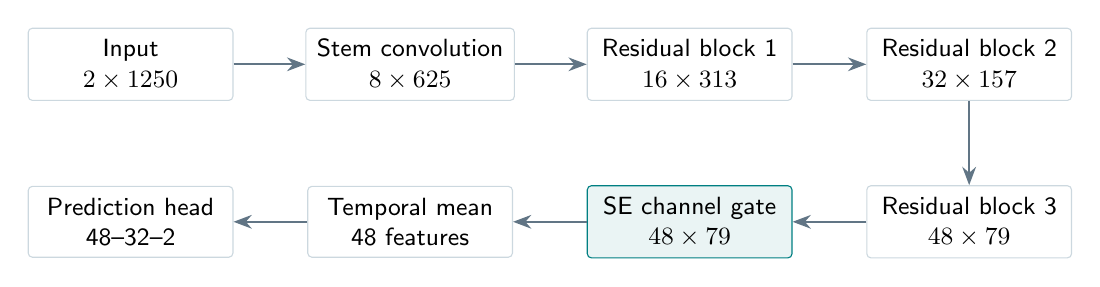
\begin{tikzpicture}[x=1cm,y=1cm]
\node[box,minimum width=2.6cm] (a) at (0,2) {Input\\$2\times1250$};
\node[box,minimum width=2.6cm] (b) at (3.55,2) {Stem convolution\\$8\times625$};
\node[box,minimum width=2.6cm] (c) at (7.1,2) {Residual block 1\\$16\times313$};
\node[box,minimum width=2.6cm] (d) at (10.65,2) {Residual block 2\\$32\times157$};
\node[box,minimum width=2.6cm] (e) at (10.65,0) {Residual block 3\\$48\times79$};
\node[accent,minimum width=2.6cm] (f) at (7.1,0) {SE channel gate\\$48\times79$};
\node[box,minimum width=2.6cm] (g) at (3.55,0) {Temporal mean\\48 features};
\node[box,minimum width=2.6cm] (h) at (0,0) {Prediction head\\48--32--2};
\foreach \s/\t in {a/b,b/c,c/d,d/e,e/f,f/g,g/h}{\draw[conn](\s)--(\t);}
\end{tikzpicture}\end{center}
\medskip Shapes show \textbf{learned feature traces $\times$ time positions}. The initial 2 means ECG and PPG. The later 48 means learned traces, not 48 sensors or people.
\takeaway{38,296 trainable parameters. Each window produces one SBP and one DBP.}
\source{[7] implementation/shared/models.py. The input retains all 1,250 samples before the learned stride-2 stem.}
\end{frame}

\begin{frame}{Convolution: a small filter scans the signal}
\begin{columns}[T]
\begin{column}{.53\textwidth}
A small learned filter slides across time. The first layer uses \textbf{7 samples per channel} at each position.
\[u_{k,t}=\sum_{c=1}^{2}\sum_{j=0}^{6}w_{k,c,j}\,x_{c,2t+j-3}.\]
\begin{itemize}\setlength\itemsep{2mm}
\item 8 filters create 8 feature traces.
\item Stride 2 moves two samples at a time.
\item Padding 3 supplies zeros at the edges.
\end{itemize}
\end{column}
\begin{column}{.43\textwidth}
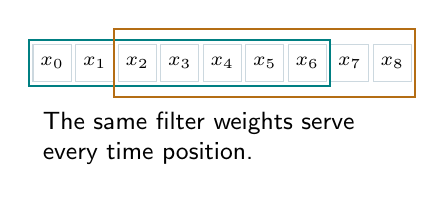
\begin{tikzpicture}[x=.54cm,y=.58cm]
\foreach \i in {0,...,8}{\draw[draw=Line] (\i,0) rectangle +(0.9,.8);\node[font=\scriptsize] at (\i+.45,.4){$x_{\i}$};}
\draw[Teal,thick](-.1,-.1) rectangle (6.99,.9);
\draw[Amber,thick](1.9,-.35) rectangle (8.99,1.15);
\node[align=left,anchor=west,font=\small,text width=4.5cm] at (0,-1.25){The same filter weights serve every time position.};
\end{tikzpicture}\par
\vspace{4mm}
\small A filter's weights are learned across many training participants. The resulting feature values depend on this particular input window.
\end{column}
\end{columns}
\source{[7] Actual stem: Conv1d(2,8,kernel=7,stride=2,padding=3,bias=False), BatchNorm, SiLU. The small diagram illustrates indexing, not measured signal values.}
\end{frame}

\begin{frame}{The small operations inside the network}
\smalltable
\begin{tabular}{P{3.2cm}P{9.6cm}}\toprule
Diagram label & Meaning\\\midrule
Conv & Convolution. A learned filter scans nearby time samples.\\[2mm]
BatchNorm & Batch normalization. It scales intermediate features using training-batch statistics and learns an adjustment.\\[2mm]
SiLU & Sigmoid Linear Unit, $u/(1+e^{-u})$. A smooth nonlinear transformation.\\[2mm]
ReLU & Rectified Linear Unit, $\max(0,u)$. It keeps positive values and sets negative values to zero.\\[2mm]
Sigmoid & A function that maps a number into the interval 0 to 1.\\[2mm]
Linear / dense & A fully connected layer. It mixes all input features using learned weights.\\\bottomrule
\end{tabular}
\source{[7] Operations in shared/models.py and paired\_se/model.py. At prediction time, batch normalization uses saved training statistics.}
\end{frame}

\begin{frame}{Inside one residual block}
\begin{center}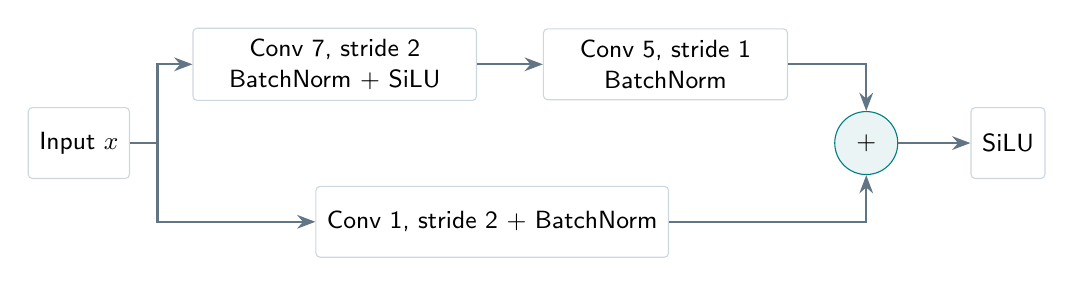
\begin{tikzpicture}[x=1cm,y=1cm]
\node[box] (x) at (0,0) {Input $x$};
\node[box,minimum width=3.6cm] (c1) at (3.25,1) {Conv 7, stride 2\\BatchNorm + SiLU};
\node[box,minimum width=3.1cm] (c2) at (7.45,1) {Conv 5, stride 1\\BatchNorm};
\node[box,minimum width=4cm] (skip) at (5.25,-1) {Conv 1, stride 2 + BatchNorm};
\node[accent,circle,minimum size=8mm] (sum) at (10,0) {$+$};
\node[box] (out) at (11.8,0) {SiLU};
\draw[conn](x.east)--++(.35,0)|-(c1.west);\draw[conn](c1)--(c2);\draw[conn](c2.east)-|(sum.north);
\draw[conn](x.east)--++(.35,0)|-(skip.west);\draw[conn](skip.east)-|(sum.south);\draw[conn](sum)--(out);
\end{tikzpicture}\end{center}
\[x_{\mathrm{next}}=\mathrm{SiLU}\big(F(x)+P(x)\big).\]
\begin{itemize}\setlength\itemsep{2mm}
\item $F(x)$ learns a transformation. $P(x)$ carries a matching shortcut.
\item The projection $P$ adjusts channel count and time length before addition.
\item Our three blocks increase channels: $8\to16\to32\to48$.
\end{itemize}
\source{[2] He et al., residual learning. [7] Our 1D kernels, projection shortcuts and SiLU implementation.}
\end{frame}

\begin{frame}{Squeeze-and-Excitation: weighting learned traces}
\begin{center}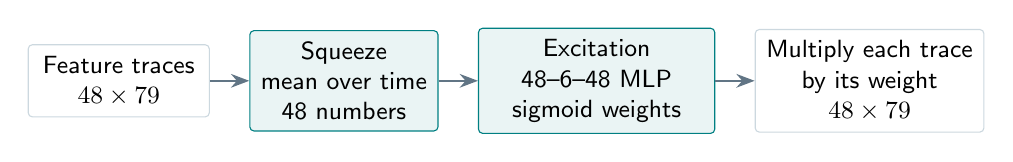
\begin{tikzpicture}[node distance=5mm]
\node[box,minimum width=2.3cm] (u) {Feature traces\\$48\times79$};
\node[accent,right=5mm of u,minimum width=2.3cm] (z) {Squeeze\\mean over time\\48 numbers};
\node[accent,right=5mm of z,minimum width=3cm] (s) {Excitation\\48--6--48 MLP\\sigmoid weights};
\node[box,right=5mm of s,minimum width=2.7cm] (o) {Multiply each trace\\by its weight\\$48\times79$};
\draw[conn](u)--(z);\draw[conn](z)--(s);\draw[conn](s)--(o);
\end{tikzpicture}\end{center}
\[z_c=\frac1{79}\sum_t U_{c,t},\qquad
 a=\mathrm{sigmoid}\!\left(W_2\,\mathrm{ReLU}(W_1z+b_1)+b_2\right),\qquad
 \widetilde U_{c,t}=a_cU_{c,t}.\]
\begin{itemize}\setlength\itemsep{2mm}
\item \textbf{Squeeze}: summarize each learned trace over the window.
\item \textbf{Excitation}: a small multilayer perceptron sets 48 weights from the summary.
\item Apply one weight to all 79 positions of the corresponding trace.
\end{itemize}
\source{[3] Hu et al., CVPR 2018. Our 1D adaptation uses temporal pooling and a reduction ratio of 8. Added parameters: 630, about 1.7\% of the plain CNN.}
\end{frame}

\begin{frame}{One person's window produces these attention weights}
\begin{columns}[T]
\begin{column}{.5\textwidth}
\begin{center}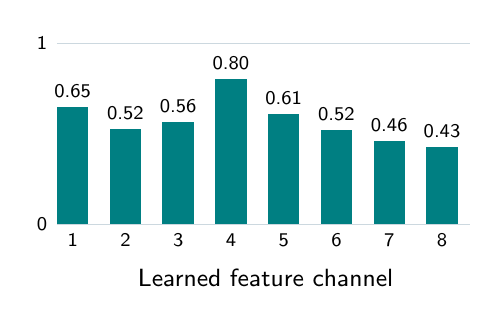
\begin{tikzpicture}[x=1cm,y=1cm]
\draw[draw=Line](0,0)--(5.25,0);\draw[draw=Line](0,2.3)--(5.25,2.3);
\node[left,font=\scriptsize]at(0,0){0};\node[left,font=\scriptsize]at(0,2.3){1};
\fill[Teal] (0.000,0) rectangle (0.400,1.493);\node[font=\scriptsize,above] at (0.200,1.493){0.65};\node[font=\scriptsize,below] at (0.200,0){1};
\fill[Teal] (0.670,0) rectangle (1.070,1.207);\node[font=\scriptsize,above] at (0.870,1.207){0.52};\node[font=\scriptsize,below] at (0.870,0){2};
\fill[Teal] (1.340,0) rectangle (1.740,1.298);\node[font=\scriptsize,above] at (1.540,1.298){0.56};\node[font=\scriptsize,below] at (1.540,0){3};
\fill[Teal] (2.010,0) rectangle (2.410,1.844);\node[font=\scriptsize,above] at (2.210,1.844){0.80};\node[font=\scriptsize,below] at (2.210,0){4};
\fill[Teal] (2.680,0) rectangle (3.080,1.396);\node[font=\scriptsize,above] at (2.880,1.396){0.61};\node[font=\scriptsize,below] at (2.880,0){5};
\fill[Teal] (3.350,0) rectangle (3.750,1.193);\node[font=\scriptsize,above] at (3.550,1.193){0.52};\node[font=\scriptsize,below] at (3.550,0){6};
\fill[Teal] (4.020,0) rectangle (4.420,1.060);\node[font=\scriptsize,above] at (4.220,1.060){0.46};\node[font=\scriptsize,below] at (4.220,0){7};
\fill[Teal] (4.690,0) rectangle (5.090,0.980);\node[font=\scriptsize,above] at (4.890,0.980){0.43};\node[font=\scriptsize,below] at (4.890,0){8};
\node[below,font=\small]at(2.65,-.45){Learned feature channel};
\end{tikzpicture}\end{center}
\end{column}
\begin{column}{.46\textwidth}
\textbf{First 8 of 48 gates}\par\medskip
The model learned its parameters from the training group. These gate values come from test person \texttt{p000053\_1}'s example window.
\begin{itemize}\setlength\itemsep{2mm}
\item Channel 4 gets a multiplier of about 0.80.
\item Channel 8 gets a multiplier of about 0.43.
\item A different input window can produce different weights.
\end{itemize}
\end{column}
\end{columns}
\takeaway{These are feature-channel weights, not ECG-versus-PPG importance scores.}
\source{[7] Saved dual-input seed-42 model. A gate is a computed value, not a newly fitted personal parameter. Channel meanings emerge during training.}
\end{frame}

\begin{frame}{Converting 48 features into two pressure estimates}
\begin{center}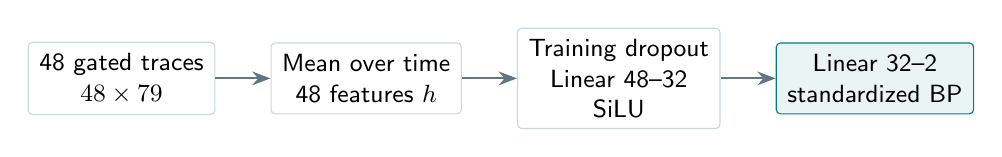
\begin{tikzpicture}[node distance=7mm]
\node[box] (a) {48 gated traces\\$48\times79$};
\node[box,right=of a] (b) {Mean over time\\48 features $h$};
\node[box,right=of b] (c) {Training dropout\\Linear 48--32\\SiLU};
\node[accent,right=of c] (d) {Linear 32--2\\standardized BP};
\draw[conn](a)--(b);\draw[conn](b)--(c);\draw[conn](c)--(d);
\end{tikzpicture}\end{center}
\[\widehat y_{\mathrm{mmHg}}=\mu+\sigma\odot\widehat y_{\mathrm{standardized}}.\]
\smalltable\begin{tabular}{lrr}\toprule
Real example & SBP & DBP\\\midrule
Network output & 0.5066 & 0.5820\\
Training-label mean $\mu$ & 115.41765 & 62.92810\\
Training-label standard deviation $\sigma$ & 18.94188 & 12.08322\\
Prediction (mmHg) & 125.01 & 69.96\\
Reference (mmHg) & 115.12 & 50.08\\\bottomrule\end{tabular}
\source{[7] Mean and standard deviation come from the group training labels. Dropout randomly sets 15\% of features to zero during training and is off during prediction. $\odot$ means multiply matching entries.}
\end{frame}

\begin{frame}{Training loss: how a wrong answer changes the model}
\textbf{Mean squared error (MSE)} averages squared prediction errors. Standardization first subtracts the training-group mean and divides by its standard deviation.
\[z_{b,d}=\frac{y_{b,d}-\mu_d}{\sigma_d},\qquad
 L=\frac1{2B}\sum_{b=1}^{B}\sum_{d\in\{\mathrm{SBP,DBP}\}}(\widehat z_{b,d}-z_{b,d})^2.\]
\begin{columns}[T]
\begin{column}{.53\textwidth}
\textbf{Why standardize the labels?}
\begin{itemize}\setlength\itemsep{2mm}
\item $B$ is the batch size. $b$ indexes a window and $d$ a pressure output.
\item Standardization sets their scales before the joint loss.
\item Squaring gives larger errors more influence on an update.
\end{itemize}
\end{column}
\begin{column}{.43\textwidth}
\textbf{One saved-model example}\par\medskip
True $z$: -0.0157 / -1.0634\\[2mm]
Predicted $z$: 0.5066 / 0.5820\\[2mm]
Two-output MSE: \textbf{1.4901}
\end{column}
\end{columns}
\source{[7] MSE is the training objective. Later slides define the separate evaluation measures. This calculation uses one test window to illustrate the arithmetic, without updating the saved model.}
\end{frame}

\begin{frame}{Stage 1: one update using the training group}
\whose{A shuffled batch from the 1,085 training people, not one target person's calibration bank.}
\begin{enumerate}\setlength\itemsep{2mm}
\item Take \textbf{256 training windows} and their supplied SBP/DBP labels.
\item Add input noise with standard deviation \textbf{0.003}.
\item Run the CNN, SE gate and readout to obtain predicted SBP/DBP.
\item Compute standardized MSE against the observed labels.
\item Backpropagation calculates how each weight affects the loss.
\item The optimizer updates the network weights using those gradients.
\end{enumerate}
\source{[7] An optimizer is the numerical rule for changing weights. Backpropagation computes gradients: how a small weight change would affect the loss.}
\end{frame}

\begin{frame}{The optimizer and training settings}
\smalltable
\begin{tabular}{P{3.6cm}P{9.1cm}}\toprule
Setting & Role and actual value\\\midrule
AdamW optimizer & Adaptive Moment Estimation with decoupled weight decay. It scales updates using past gradients.\\[2mm]
Learning rate & Overall update size: \textbf{0.001}.\\
Weight decay & Shrinks weights during group training: \textbf{0.001}.\\
Gradient clipping & Caps the total gradient norm at \textbf{5} to limit a large update.\\
Batch size & \textbf{256 windows} per step.\\
Training loss & Mean squared error of the two standardized BP labels.\\\bottomrule
\end{tabular}
\par\medskip The validation group selects checkpoints. Its labels do not contribute optimizer updates.
\source{[7] attention\_cnn/train.py. The personal optimizer later uses Adam without weight decay.}
\end{frame}

\begin{frame}{How long group training actually ran}
\begin{columns}[T]
\begin{column}{.48\textwidth}
\begin{itemize}\setlength\itemsep{3mm}
\item Maximum: \textbf{40 epochs}.
\item Stop after \textbf{8 epochs} without validation improvement.
\item Halve learning rate after \textbf{3} validation non-improvements.
\item Score: mean absolute error (\textbf{MAE}), averaged first per person, then across people and the two pressures.
\end{itemize}
\end{column}
\begin{column}{.49\textwidth}
\smalltable\begin{tabular}{lrrrr}\toprule
Input & Seed & Run & Best & Val. MAE\\\midrule
dual & 42 & 9 & 1 & 10.291\\
dual & 43 & 9 & 1 & 10.457\\
dual & 44 & 9 & 1 & 10.421\\
ppg & 42 & 9 & 1 & 10.374\\
ppg & 43 & 9 & 1 & 10.583\\
ppg & 44 & 9 & 1 & 10.406\\
\bottomrule\end{tabular}
\par\medskip\small All six fits ran \textbf{9 epochs} and retained \textbf{epoch 1}. Additional epochs did not improve this validation criterion.
\end{column}
\end{columns}
\source{[7] Recorded completions. Run and Best are epoch numbers. Three seeds describe fitting variation, not three independent participant cohorts.}
\end{frame}

\begin{frame}{Two separately trained group models}
\begin{center}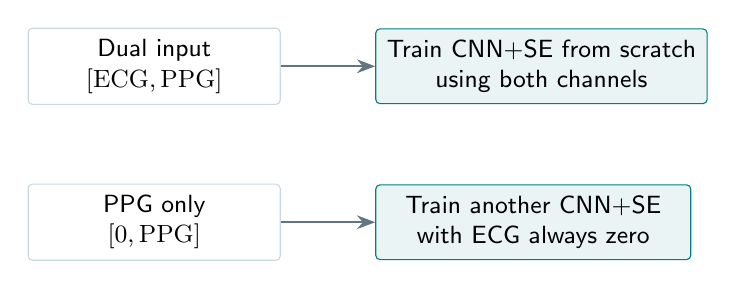
\begin{tikzpicture}
\node[box,minimum width=3.2cm] (d) {Dual input\\$[\mathrm{ECG},\mathrm{PPG}]$};
\node[accent,right=12mm of d,minimum width=4.0cm] (a) {Train CNN+SE from scratch\\using both channels};
\node[box,below=10mm of d,minimum width=3.2cm] (p) {PPG only\\$[0,\mathrm{PPG}]$};
\node[accent,right=12mm of p,minimum width=4.0cm] (b) {Train another CNN+SE\\with ECG always zero};
\draw[conn](d)--(a);\draw[conn](p)--(b);
\end{tikzpicture}\end{center}
\begin{itemize}\setlength\itemsep{2mm}
\item Both have \textbf{38,296 parameters}, identical settings and seeds 42/43/44.
\item The PPG-only model learns without ECG throughout training.
\item Its internal input mask also applies inside the personal reference encoder.
\end{itemize}
\source{[7] implementation/modality\_se/model.py. Keeping two tensor slots makes the architecture comparison parameter-matched. The PPG inference wrapper can accept a single channel.}
\end{frame}

\begin{frame}{Why this group architecture?}
\smalltable
\begin{tabular}{P{2.7cm}P{4.4cm}P{5.6cm}}\toprule
Source & Published idea & Our adaptation\\\midrule
Our V1 baseline & Learn from complete signal windows & Keep all 1,250 input samples before learned downsampling\\[2mm]
He et al. [2] & Residual learning: a shortcut around a transformation & Three compact one-dimensional blocks, widths 16, 32, 48\\[2mm]
Hu et al. [3] & Squeeze-and-Excitation: weight feature channels & One gate after the final block, with a 48--6--48 network\\\bottomrule
\end{tabular}
\takeaway{We combine published building blocks with our own compact signal model.}
\source{[2,3,7] These are adaptations of ideas, not reproductions of the original image-classification architectures. The six-architecture comparison appears in the results section.}
\end{frame}

\stage{Personalization: one target person's early and later data}
\begin{frame}{One person's timeline}

\whose{Only person P. All 30 personal pipelines repeat this procedure independently.}
\begin{center}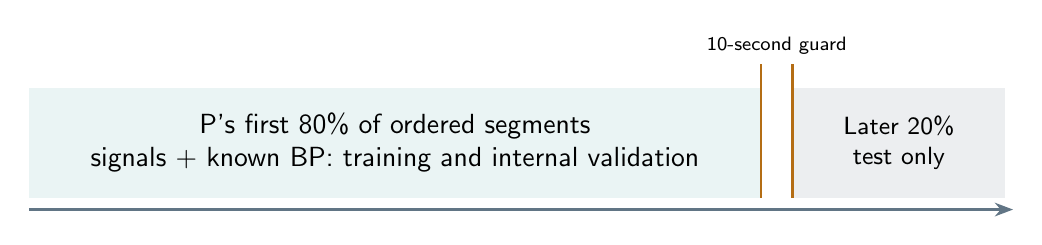
\begin{tikzpicture}[x=1cm,y=1cm]
\fill[Pale](0,0)rectangle(9.3,1.4);\fill[Navy!8](9.7,0)rectangle(12.4,1.4);
\node[align=center,text width=8.7cm]at(4.65,.7){P's first 80\% of ordered segments\\signals + known BP: training and internal validation};
\node[align=center,text width=2.4cm,font=\small]at(11.05,.7){Later 20\%\\test only};
\draw[Amber,thick](9.3,0)--(9.3,1.7);\draw[Amber,thick](9.7,0)--(9.7,1.7);
\node[above,font=\scriptsize]at(9.5,1.7){10-second guard};
\draw[conn](0,-.15)--(12.5,-.15);
\end{tikzpicture}\end{center}
\begin{itemize}\setlength\itemsep{3mm}
\item The \textbf{reference bank} stores P's development waveforms and known SBP/DBP.
\item Three time-ordered validation periods inside the 80\% choose P's settings.
\item After selection, refit on all of P's development bank, then freeze the model.
\end{itemize}
\source{[7] 20261015 protocol: chronological segment-count split, not a random split or the previous 20\%-of-elapsed-time support rule. Later true BP is available only to the scoring code.}

\end{frame}

\begin{frame}{PairSE compares two windows from the same person}
\begin{center}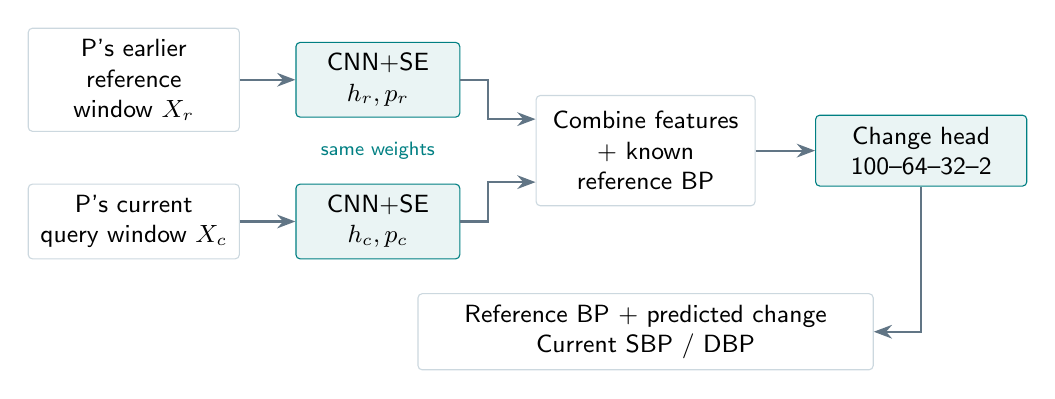
\begin{tikzpicture}[x=1cm,y=1cm]
\node[box,text width=2.4cm] (r) at(0,1.2){P's earlier\\reference window $X_r$};
\node[box,text width=2.4cm] (c) at(0,-.6){P's current\\query window $X_c$};
\node[accent,text width=1.8cm] (er) at(3.1,1.2){CNN+SE\\$h_r,p_r$};
\node[accent,text width=1.8cm] (ec) at(3.1,-.6){CNN+SE\\$h_c,p_c$};
\node[font=\scriptsize,text=Teal] at(3.1,.3){same weights};
\node[box,text width=2.5cm,minimum height=14mm] (feat) at(6.5,.3){Combine features\\+ known\\reference BP};
\node[accent,text width=2.4cm] (head) at(10.0,.3){Change head\\100--64--32--2};
\node[box,text width=5.5cm] (out) at(6.5,-2){Reference BP + predicted change\\Current SBP / DBP};
\draw[conn](r)--(er);\draw[conn](c)--(ec);\draw[conn](er.east)--++(.35,0)|-([yshift=4mm]feat.west);\draw[conn](ec.east)--++(.35,0)|-([yshift=-4mm]feat.west);
\draw[conn](feat)--(head);\draw[conn](head.south)|-(out.east);
\end{tikzpicture}\end{center}
\small $h$ contains \textbf{48 learned features}. $p$ contains \textbf{two group-model pressure estimates}. Subscript $r$ means reference and $c$ means current.
\takeaway{The reference tells the model this person's known BP at a known signal state.}
\source{[4,5] Related paired-measurement and reference-change ideas. [7] Our shared CNN+SE and PairSE implementation. Both branches reuse one encoder, not two independently trained networks.}
\end{frame}

\begin{frame}{What goes into the 100-dimensional change head?}
{\small\color{Teal}One reference and one current window from the same person.}\par\smallskip
\smalltable\begin{tabular}{P{3cm}rP{8.1cm}}\toprule
Component & Size & Information supplied\\\midrule
$h_c-h_r$ & 48 & How the current waveform features differ from the reference\\[1mm]
$h_r$ & 48 & The reference signal's feature state\\[1mm]
$y_r$ & 2 & Known reference SBP and DBP, standardized\\[1mm]
$p_c-p_r$ & 2 & The original model's expected BP change\\\midrule
Concatenated input & \textbf{100} & $48+48+2+2$\\\bottomrule\end{tabular}
\medskip
\[g_\phi:\quad100\xrightarrow{\mathrm{Linear+SiLU}}64
\xrightarrow{\mathrm{Linear+SiLU}}32\xrightarrow{\mathrm{Linear}}2.\]
\small We join the four groups of numbers in order. Feature scaling uses statistics learned from the training group. A 0.01 minimum scale avoids dividing by a very small number.
\par\smallskip{\color{Teal}\bfseries 8,610 change-head parameters; 46,906 in full PairSE.}
\source{[7] implementation/paired\_se/model.py. Feature vectors in this slide denote standardized encoder features. BP uses its own source-label mean and SD.}
\end{frame}

\begin{frame}{The prediction equation, one term at a time}
\small All terms describe \textbf{the same person}. $y_r$ is their measured earlier BP. $p_r,p_c$ are the shared model's earlier/current predictions. $g_\phi$ is the small change network with weights $\phi$.
\[\boxed{\widehat y_{c\mid r}=\underbrace{y_r}_{\text{known BP}}+
\underbrace{(p_c-p_r)}_{\text{base-model change}}+
\underbrace{g_\phi(z_{cr})-g_\phi(z_{rr})}_{\text{learned change correction}}}\]
\[z_{cr}=[h_c-h_r,h_r,y_r,p_c-p_r],\qquad z_{rr}=[0,h_r,y_r,0].\]
\begin{itemize}\setlength\itemsep{2mm}
\item $g_\phi(z_{cr})$ learns a correction from the current/reference pair.
\item $g_\phi(z_{rr})$ uses the reference as both inputs: an identity anchor.
\item If $X_c=X_r$, both change terms cancel, giving exactly $\widehat y_{c\mid r}=y_r$.
\end{itemize}
\takeaway{Predict a change relative to a known measurement, rather than relearning absolute BP from scratch.}
\source{[7] This equation and identity subtraction are our implemented design. BP terms use source-label standardization; encoder features use their own source statistics.}
\end{frame}

\begin{frame}{How the design includes simple bias correction}
\small Before group pair training, we set the change network's last layer to zero. Then $g_\phi=0$ and one same-person pair predicts
\[\widehat y_{c\mid r}=y_r+p_c-p_r.\]
At prediction time, average over this person's $K$ early references:
\[\frac1K\sum_r\big[y_r+p_c-p_r\big]=p_c+\frac1K\sum_r(y_r-p_r).\]
\begin{itemize}\setlength\itemsep{3mm}
\item $K$ is the number of reference windows from this person.
\item The right-hand side is \textbf{simple personal bias correction}: add this person's average earlier prediction error to the current estimate.
\item Training can then learn a \textbf{waveform-dependent} adjustment to that starting point.
\end{itemize}
\takeaway{PairSE adds a waveform-dependent adjustment to ordinary bias correction.}
\source{[7] The equality explains source-head initialization. It does not guarantee that source training or personal fitting will outperform the bias baseline.}
\end{frame}

\begin{frame}{Our adaptation of the paired-measurement idea}
\small Mekonnen et al. call their method \textbf{Mixed Deduction Learning (MDL)}. It is the paper that directly inspired our reference/current pairing [4].
\par\smallskip
\smalltable\begin{tabular}{P{3.0cm}P{4.6cm}P{5.3cm}}\toprule
Design aspect & Mekonnen et al. [4] & Our PairSE [7]\\\midrule
Paired inputs & Earlier and later PPG measurements & Reference/current ECG+PPG or PPG-only windows\\[2mm]
Meaning of two channels & Two PPG recordings in a measurement pair & ECG and PPG are sensor channels inside each window\\[2mm]
Training strategy & Mix personal calibration data with other subjects' data & Pretrain encoder, train source pair head, then adapt the personal tail and head\\[2mm]
Network design & Their CNN-based mixed deduction model & Shared residual CNN+SE plus a 100-D change MLP\\[2mm]
Prediction construction & Learn from paired measurements & Explicit reference BP, identity subtraction, all-reference averaging\\\bottomrule\end{tabular}
\source{[4,7] Direct inspiration, with our own architecture and evaluation. Related work: Schlesinger et al. [5] study reference-based BP changes, and Leitner et al. [6] study transfer to individuals.}
\end{frame}

\stage{Stage 2: train a shared change head on the group}
\begin{frame}{Stage 2 still uses the group, not a target person}
\whose{The same 1,085 training people. Every pair stays within one of those people.}
\begin{enumerate}\setlength\itemsep{2mm}
\item Start from the saved population CNN+SE and \textbf{freeze its weights}.
\item Save 48 features and two pressure predictions for each training window.
\item For each training window, randomly choose a \textbf{different window from the same person} as its reference.
\item Give PairSE the reference's BP. Use the current window's BP as the loss target.
\item Train only the change head: Adam optimizer, learning rate \textbf{0.001}, batch \textbf{2,048}, standardized mean squared error, gradient clip \textbf{5}.
\item Choose a checkpoint using fixed validation pairs, up to \textbf{20 epochs} with patience \textbf{5}.
\end{enumerate}
\source{[7] paired\_se/run.py. Each epoch visits 390,600 training windows. These group subset files lack timestamps, so pair order here is not chronological. Adam means Adaptive Moment Estimation.}
\end{frame}

\begin{frame}{Same-person pairs can still train a group model}
\begin{center}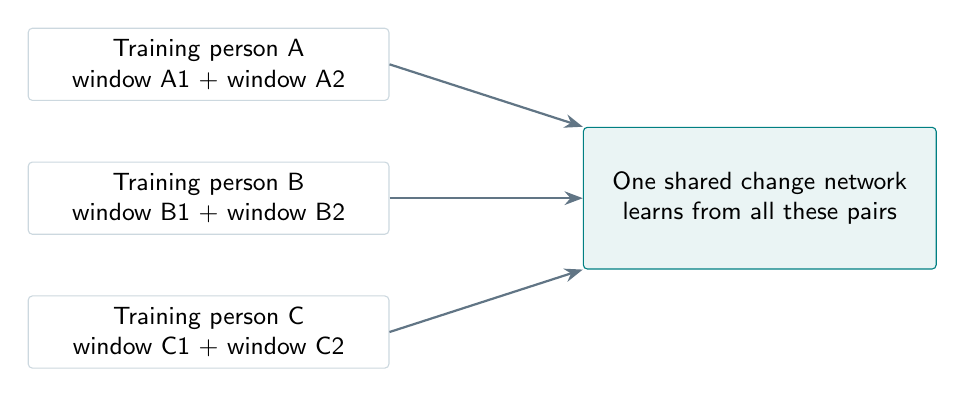
\begin{tikzpicture}[x=1cm,y=1cm]
\node[box,text width=4.3cm] (a) at(0,1.7){Training person A\\window A1 + window A2};
\node[box,text width=4.3cm] (b) at(0,0){Training person B\\window B1 + window B2};
\node[box,text width=4.3cm] (c) at(0,-1.7){Training person C\\window C1 + window C2};
\node[accent,text width=4.2cm,minimum height=18mm] (m) at(7.0,0){One shared change network\\learns from all these pairs};
\draw[conn](a.east)--(m.north west);\draw[conn](b.east)--(m.west);\draw[conn](c.east)--(m.south west);
\end{tikzpicture}\end{center}
\takeaway{Within a pair: one person. Across training: many people.}
\source{[7] Illustrative participants A/B/C show the implemented pairing rule. A pair never combines A's known pressure with B's current waveform.}
\end{frame}

\begin{frame}{Group pair training: actual completed epochs}
\begin{center}
\begin{tabular}{llrr}\toprule
Input mode & Seed & Epochs run & Best epoch\\\midrule
ECG+PPG & 42 & 20 & 18\\
ECG+PPG & 43 & 17 & 12\\
ECG+PPG & 44 & 16 & 11\\\midrule
PPG-only & 42 & 20 & 16\\
PPG-only & 43 & 20 & 15\\
PPG-only & 44 & 20 & 20\\\bottomrule
\end{tabular}
\end{center}
\takeaway{The population backbone and the pair head have separate training schedules.}
\small These epochs use the group dataset. The next stage chooses the update count separately for each target person and pressure, using only their early data.
\source{[7] Saved source-head completion records in paired\_se/population and modality\_se/pair\_population. Each checkpoint is selected on source validation pairs.}
\end{frame}

\stage{Stage 3: fit one copy using only person P's early data}
\begin{frame}{Stage 3: one independent model copy per person}
\begin{center}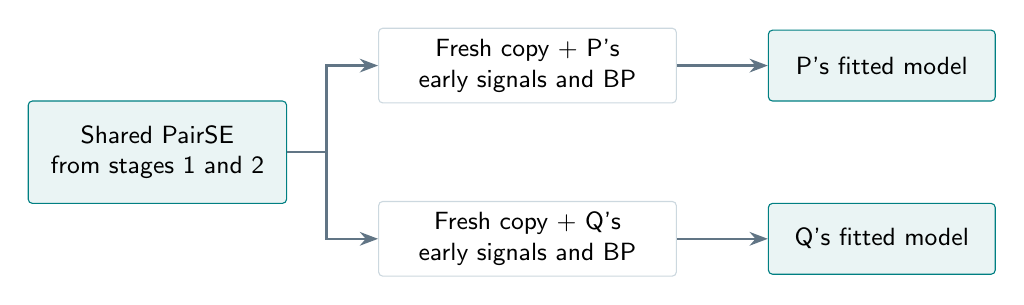
\begin{tikzpicture}[x=1cm,y=1cm]
\node[accent,text width=3.0cm,minimum height=13mm] (g) at(0,0){Shared PairSE\\from stages 1 and 2};
\node[box,text width=3.5cm] (a) at(4.7,1.1){Fresh copy + P's\\early signals and BP};
\node[box,text width=3.5cm] (b) at(4.7,-1.1){Fresh copy + Q's\\early signals and BP};
\node[accent,text width=2.6cm] (ap) at(9.2,1.1){P's fitted model};
\node[accent,text width=2.6cm] (bp) at(9.2,-1.1){Q's fitted model};
\draw[conn](g.east)--++(.5,0)|-(a.west);\draw[conn](g.east)--++(.5,0)|-(b.west);
\draw[conn](a)--(ap);\draw[conn](b)--(bp);
\end{tikzpicture}\end{center}
\begin{itemize}\setlength\itemsep{3mm}
\item P's updates affect only P's copy. Q starts from the same group checkpoint.
\item Each person keeps their own early reference bank for later predictions.
\end{itemize}
\source{[7] This is the target-person fitting procedure. It does not sequentially continue P's personalized weights on Q.}
\end{frame}

\begin{frame}{Exactly what changes during personal fitting}

\whose{Only this target person's development pairs; the starting weights come from the group.}
\smalltable\begin{tabular}{P{4.7cm}P{8cm}}\toprule
Component & During this person's fitting\\\midrule
Stem + residual blocks 1 and 2 & Frozen weights\\
Last residual CNN block & \textbf{Trainable} signal features\\
Last SE channel-attention gate & \textbf{Trainable} feature-channel weighting\\
Reference-conditioned change head & \textbf{Trainable} 100--64--32--2 network\\
Population readout weights & Frozen, but its input features can change\\
Label/feature scaling, BatchNorm statistics & Frozen; dropout disabled\\\bottomrule
\end{tabular}
\takeaway{33,336 trainable parameters per endpoint copy; 46,906 in full PairSE.}
\source{[7] Trainable names: change.*, encoder.body.6.*, encoder.gates.6.*. BatchNorm affine scale/bias in the last block can train. SE = Squeeze-and-Excitation; CNN = convolutional neural network.}

\end{frame}

\stage{Personal settings: chosen separately within each person}
\begin{frame}{Each person chooses their own fitting settings}

\whose{Only P's first 80\%. No other target person chooses P's hyperparameters.}
\smalltable\begin{tabular}{lrr}\toprule
Internal period & Train on development bank & Validate on development bank\\\midrule
1 & First 50\% & Next 15\% (50--65\%)\\
2 & First 65\% & Next 15\% (65--80\%)\\
3 & First 80\% & Last 20\% (80--100\%)\\\bottomrule
\end{tabular}
\par\medskip\textbf{These percentages are inside P's development bank.} P's final test 20\% is outside this entire procedure.
\begin{itemize}\setlength\itemsep{2mm}
\item Tail learning rate: \textbf{0.0001 or 0.0003}. Updates: \textbf{10,25,50,100}.
\item Also compare zero extra updates; every candidate starts from the source model.
\item Select SBP and DBP settings separately by mean MAE over the three periods.
\end{itemize}
\source{[7] Ten-second guards at validation boundaries. Ties favor fewer updates, then lower learning rate. Hyperparameters are settings, not fitted weights. MAE = mean absolute error.}

\end{frame}

\begin{frame}{From selected settings to a fitted personal model}

\begin{enumerate}\setlength\itemsep{3mm}
\item Save P's selected learning rate and number of updates for \textbf{SBP}.
\item Save P's separately selected settings for \textbf{DBP}.
\item Restart two copies of the same source model. Fit each endpoint on \textbf{all of P's development bank} using its chosen settings.
\item Each Adam step uses \textbf{every valid chronological reference/current pair}; reference end + 10 seconds must precede current start.
\item Optimize that endpoint's standardized MSE; clip gradient norm at 5; no weight decay.
\end{enumerate}
\takeaway{Two endpoint checkpoints per person and source seed, using one tail-adaptation policy.}
\source{MSE = mean squared error. Adam = Adaptive Moment Estimation. The candidate with zero updates remains possible. The reference bank stays separate from the weights.}

\end{frame}

\stage{Stage 4: frozen personal model predicts P's later pressure}
\begin{frame}{What is available at a later prediction time?}
\whose{The same person P, now at a later time. Fitting has finished.}
\smalltable
\begin{tabular}{P{4.2cm}P{8.4cm}}\toprule
Available to the predictor & Role\\\midrule
P's current ECG/PPG & The signal whose corresponding pressure we estimate\\[2mm]
P's saved early signals & Reference waveform states\\[2mm]
P's saved early SBP/DBP & Known pressures at those earlier states\\[2mm]
P's fitted model weights & Convert each reference/current pair into an estimate\\\bottomrule
\end{tabular}
\par\medskip We average estimates over all eligible early references. The evaluation code then compares the output with P's \textbf{later true BP}, which the predictor never receives.
\takeaway{We observe the later ECG/PPG. The earlier 80\% calibrates the model; the later signals are observed inputs.}
\source{[7] Saved personal weights and the separate personal reference bank jointly define the deployed personal predictor.}
\end{frame}

\begin{frame}{A real tail-adapted prediction, step by step}
\small Person \texttt{p000006}, dual-input seed 42. First reference row 0; first eligible test row 97. This person's two endpoints each selected learning rate 0.0003 and 25 updates.
\par\medskip\smalltable
\begin{tabular}{P{9.3cm}r}\toprule
Quantity & SBP / DBP (mmHg)\\\midrule
Known reference BP $y_r$ & 108.29 / 66.40\\
Readout change $p_c-p_r$ after tail adaptation & -2.33 / -4.55\\
Learned change correction, converted to mmHg & -20.32 / -14.14\\\midrule
Prediction using this one reference & 85.64 / 47.71\\
Actual inference: average over all 96 early references & \textbf{92.44 / 47.95}\\
True BP for the later query, used only for scoring & 93.10 / 50.36\\\bottomrule
\end{tabular}
\par\medskip This early bank supplies \textbf{4,488 valid pairs} per fitting step. Pairing reuses observed labels; it does not create new independent measurements.
\source{[7] Replayed 20261015 tail checkpoints. Example chosen by participant/row order, not by error. Each endpoint uses its own selected copy; arithmetic is converted from standardized BP to mmHg.}
\end{frame}

\begin{frame}{The two simple controls use exactly the same data}
\textbf{Personal mean: one constant prediction for this person}
\[\widehat y_c^{\mathrm{mean}}=\frac1K\sum_r y_r.\]
\textbf{Bias correction: retain the population prediction's changes}
\[\widehat y_c^{\mathrm{bias}}=p(X_c)+\frac1K\sum_r\left[y_r-p(X_r)\right].\]
\smalltable\begin{tabular}{lr}\toprule
Same real query as the previous slide & SBP / DBP (mmHg)\\\midrule
Personal mean & 94.97 / 49.00\\
Population prediction + personal bias & 95.34 / 46.18\\
Tail-adapted PairSE with the same reference bank & 92.44 / 47.95\\\bottomrule\end{tabular}
\takeaway{Every method gets the same early labels, later queries and input modality.}
\source{[7] Personal mean ignores query waveforms. Bias correction uses the modality's own pretrained model. Aggregate results, rather than this one example, decide the comparison.}
\end{frame}

\stage{Results: metric definitions}
\begin{frame}{How we measure prediction error}
\smalltable\begin{tabular}{P{3.3cm}P{7.6cm}l}\toprule
Metric & Question answered & Better\\\midrule
MAE: mean absolute error & Average absolute error in mmHg & Lower\\
RMSE: root mean squared error & Square errors, average them, then take the square root & Lower\\
Signed Bias & Systematic overprediction or underprediction & Closer to 0\\
Error SD: standard deviation & Variation of errors around their mean & Lower\\
Within $\pm5/10/15$ & Percentage of estimates close to the reference & Higher\\
Participant-macro MAE & Average each person's MAE, then weight people equally & Lower\\\bottomrule\end{tabular}
\par\medskip\textbf{Macro versus pooled:} macro weights participants equally. Pooled weights every window equally. Macro SD averages within-person SD.
\par\medskip We report the mean of \textbf{three separate seeds}, not predictions from a three-model ensemble.
\source{[7] shared/metrics.py. SD uses the sample denominator n-1. These metrics characterize our dataset errors and do not establish clinical-device certification.}
\end{frame}

\stage{Group model results: no personal calibration}
\begin{frame}{Group models: six matched architectures}
\small Validation: \textbf{192 people}. Main test: \textbf{141 people}. Each saved group model predicts all their windows without personal fitting.
\par\smallskip
\smalltable\begin{tabular}{lrr}\toprule
Architecture & Validation MAE & Main-test MAE\\\midrule
Plain residual CNN & \textbf{12.41} / 8.33 & 12.59 / 8.36\\
CNN + SE & 12.51 / \textbf{8.26} & \textbf{12.39} / \textbf{8.00}\\
CNN + temporal gate & 12.49 / 8.32 & 12.58 / 8.31\\
CNN + CBAM & 12.52 / 8.29 & 12.42 / 8.11\\
CNN + additive gate & 12.44 / 8.34 & 12.66 / 8.18\\
CNN + SE at all stages & 12.47 / 8.32 & 12.49 / 8.23\\
\bottomrule\end{tabular}
\par\smallskip\scriptsize SBP / DBP, mmHg. Bold: lowest MAE for each endpoint within each partition.
\par\smallskip\small\textbf{Observed test comparison:} CNN+SE improves MAE from 12.59/8.36 to 12.39/8.00 mmHg.
\par\smallskip\textbf{Selection context:} plain CNN has the slightly better mean validation score; SE is our retained V2 backbone, not the winner of every ranking.
\source{[7] Three-seed mean absolute errors on the same corrected splits. CBAM means Convolutional Block Attention Module. Temporal and additive gates are alternative weighting modules. Bold indicates numerical rank.}
\end{frame}

\begin{frame}{Group models: two signals versus one signal}
\smalltable\begin{tabular}{lrr}\toprule
Main-test pooled metric & ECG+PPG CNN+SE & PPG-only CNN+SE\\\midrule
MAE & 12.39 / 8.00 & \textbf{12.32} / \textbf{7.85}\\
RMSE & 15.89 / 10.19 & \textbf{15.73} / \textbf{9.88}\\
Bias & \textbf{-1.76} / \textbf{-0.89} & -2.05 / -1.64\\
Error SD & 15.78 / 10.15 & \textbf{15.57} / \textbf{9.67}\\
$\leq5$ (\%) & \textbf{26.03} / \textbf{38.83} & 25.52 / 38.39\\
$\leq10$ (\%) & \textbf{49.22} / 68.91 & 48.67 / \textbf{69.38}\\
$\leq15$ (\%) & 67.60 / 86.68 & \textbf{67.82} / \textbf{87.85}\\
\bottomrule\end{tabular}
\metricnote
\par\medskip\normalsize PPG-only has slightly lower main-test MAE. Dual input has Bias closer to zero and the better validation score within the SE family.
\par\smallskip On the separate AAMI-designated stress subset, macro MAE is \textbf{19.99/12.62} for dual versus \textbf{20.80/13.19} for PPG-only.
\source{[7] Three-seed averages. Neither input mode wins every metric or dataset. We retain both.}
\end{frame}

\stage{Current personal results: 30 people, later 20\% test}
\begin{frame}{Matched comparison: all 30 people}
\small Equal-person MAE, then average of three seeds. Values are SBP / DBP, mmHg.\par\medskip\begin{tabular}{lrr}\toprule Method & PPG only & ECG+PPG\\\midrule
Population (no calibration) & 14.66 / 10.60 & 14.80 / 10.35\\
Personal mean & 12.24 / 6.02 & 12.24 / 6.02\\
Bias correction & 8.51 / 5.38 & 9.09 / 5.70\\
Fixed PairSE & 7.75 / 4.80 & 8.78 / 5.05\\
Single-period selection & 7.72 / 4.67 & 8.17 / 4.78\\
Head-only adaptation & 7.59 / 4.54 & 8.39 / 4.89\\
Tail adaptation (adopted) & \textbf{6.89 / 4.29} & \textbf{7.14 / 4.31}\\
Scope selection (comparison) & 7.15 / 4.23 & 7.23 / 4.52\\
\bottomrule\end{tabular}\takeaway{Adopted: tail adaptation, with each person selecting their own settings.}\source{Bold identifies the adopted method here; this is not a claim that it wins every endpoint. Scope selection has slightly lower PPG DBP MAE. All controls use matched calibration/test records.}
\end{frame}
\begin{frame}{How much does the adopted method improve?}
\begin{center}\begin{tabular}{lrr}\toprule Comparison & MAE reduction (mmHg) & Relative reduction\\\midrule
PPG only vs Personal mean & 5.35 / 1.73 & 43.70 / 28.77\%\\
PPG only vs Bias correction & 1.62 / 1.09 & 19.00 / 20.34\%\\
ECG+PPG vs Personal mean & 5.11 / 1.71 & 41.71 / 28.37\%\\
ECG+PPG vs Bias correction & 1.96 / 1.39 & 21.54 / 24.37\%\\\bottomrule\end{tabular}\end{center}\takeaway{Both pressures improve in the overall 30-person mean in every source seed.}\small This is an overall result, not a guarantee for every participant.\source{Same participant weighting and same development/test records for each comparison; SBP / DBP.}
\end{frame}
\begin{frame}{PPG only: full metric panel}
\smalltable
\begin{tabular}{lrrr}\toprule
Metric & Personal mean & Bias correction & Tail adaptation\\\midrule
MAE & 12.24 / 6.02 & 8.51 / 5.38 & \textbf{6.89} / \textbf{4.29}\\
RMSE & 14.32 / 7.11 & 10.12 / 6.17 & \textbf{8.51} / \textbf{5.16}\\
Signed Bias & -6.07 / -2.80 & -2.81 / -1.48 & \textbf{-0.70} / \textbf{-0.74}\\
Sample error SD & 9.13 / 4.69 & 7.12 / 3.89 & \textbf{6.52} / \textbf{3.68}\\
$\leq5$ (\%) & 31.14 / 58.60 & 42.98 / 59.35 & \textbf{47.14} / \textbf{65.91}\\
$\leq10$ (\%) & 56.26 / 81.76 & 70.29 / 86.43 & \textbf{75.87} / \textbf{92.65}\\
$\leq15$ (\%) & 72.42 / 89.22 & 85.07 / 94.18 & \textbf{90.50} / \textbf{98.91}\\
\bottomrule\end{tabular}\metricnote\takeaway{Tail adaptation improves both errors and coverage relative to matched controls.}\source{Thirty participants, three source seeds. Error SD is averaged within person; pooled results are reported separately in the IEEE report.}
\end{frame}
\begin{frame}{PPG only: does the result repeat across seeds?}
\begin{center}\smalltable\begin{tabular}{lrrr}\toprule Method & Seed 42 & Seed 43 & Seed 44\\\midrule
Personal mean & 12.24 / 6.02 & 12.24 / 6.02 & 12.24 / 6.02\\
Bias correction & 8.45 / 5.37 & 8.58 / 5.32 & 8.50 / 5.45\\
Head only & 7.84 / 4.45 & 7.81 / 4.94 & 7.13 / 4.23\\
Tail adaptation & 7.31 / 4.43 & 6.68 / 4.25 & 6.69 / 4.18\\
Scope selection & 7.41 / 4.32 & 7.22 / 4.29 & 6.82 / 4.10\\
\bottomrule\end{tabular}\end{center}\takeaway{Tail adaptation beats both baselines on both pressures in every seed.}\small Tail MAE standard deviation across seeds: 0.36 / 0.13 mmHg.\source{Seeds change source training randomness, not participants, splits or budgets. Results are separate runs, not an ensemble.}
\end{frame}
\begin{frame}{ECG+PPG: full metric panel}
\smalltable
\begin{tabular}{lrrr}\toprule
Metric & Personal mean & Bias correction & Tail adaptation\\\midrule
MAE & 12.24 / 6.02 & 9.09 / 5.70 & \textbf{7.14} / \textbf{4.31}\\
RMSE & 14.32 / 7.11 & 10.86 / 6.54 & \textbf{8.86} / \textbf{5.22}\\
Signed Bias & -6.07 / -2.80 & -2.54 / -1.26 & \textbf{-1.57} / \textbf{-0.77}\\
Sample error SD & 9.13 / 4.69 & 8.11 / 4.52 & \textbf{7.18} / \textbf{4.00}\\
$\leq5$ (\%) & 31.14 / 58.60 & 39.95 / 55.02 & \textbf{47.01} / \textbf{66.76}\\
$\leq10$ (\%) & 56.26 / 81.76 & 66.51 / 84.10 & \textbf{74.28} / \textbf{92.23}\\
$\leq15$ (\%) & 72.42 / 89.22 & 82.24 / 94.19 & \textbf{88.56} / \textbf{98.42}\\
\bottomrule\end{tabular}\metricnote\takeaway{Tail adaptation improves both errors and coverage relative to matched controls.}\source{Thirty participants, three source seeds. Error SD is averaged within person; pooled results are reported separately in the IEEE report.}
\end{frame}
\begin{frame}{ECG+PPG: does the result repeat across seeds?}
\begin{center}\smalltable\begin{tabular}{lrrr}\toprule Method & Seed 42 & Seed 43 & Seed 44\\\midrule
Personal mean & 12.24 / 6.02 & 12.24 / 6.02 & 12.24 / 6.02\\
Bias correction & 9.01 / 5.65 & 8.88 / 5.55 & 9.39 / 5.90\\
Head only & 7.94 / 4.71 & 8.95 / 4.85 & 8.28 / 5.12\\
Tail adaptation & 7.16 / 4.44 & 7.23 / 4.26 & 7.01 / 4.23\\
Scope selection & 7.38 / 4.58 & 7.38 / 4.44 & 6.94 / 4.53\\
\bottomrule\end{tabular}\end{center}\takeaway{Tail adaptation beats both baselines on both pressures in every seed.}\small Tail MAE standard deviation across seeds: 0.11 / 0.11 mmHg.\source{Seeds change source training randomness, not participants, splits or budgets. Results are separate runs, not an ensemble.}
\end{frame}
\begin{frame}{Tail adaptation versus choosing the scope}

\textbf{Adopted method:} fix the trainable components to the change head + last CNN block + SE. Each person still selects learning rate and update count.
\par\medskip
\textbf{Scope-selection comparator:} additionally let internal validation choose head-only or tail fitting. This was tested, but is not our retained policy.
\par\medskip
\begin{tabular}{lrr}\toprule Policy & PPG MAE & Dual MAE\\\midrule
Head-only selection & 7.59 / 4.54 & 8.39 / 4.89\\
Tail selection (adopted) & 6.89 / 4.29 & 7.14 / 4.31\\
Head/tail scope selection & 7.15 / 4.23 & 7.23 / 4.52\\\bottomrule\end{tabular}
\takeaway{Personal hyperparameter selection does not require changing the trainable scope.}
\source{SBP / DBP, mmHg. Both strategies allow a validation-selected zero-update source checkpoint. The latter is a fallback, not a third learned architecture.}

\end{frame}
\begin{frame}{Overall gains and individual outcomes answer different questions}

\smalltable\begin{tabular}{lrr}\toprule Strict wins over both controls, both pressures & PPG & ECG+PPG\\\midrule
Seed 42 / 43 / 44 & 11 / 9 / 7 & 12 / 12 / 15\\
After averaging each person's MAE across seeds & 10 / 30 & 13 / 30\\
The same person wins in all three seeds & 3 / 30 & 10 / 30\\\bottomrule\end{tabular}
\par\medskip
\begin{itemize}\setlength\itemsep{3mm}
\item The overall mean improves in all seeds even though some individuals worsen.
\item Removing the largest beneficiary as a sensitivity check still gives tail-minus-bias MAE of -0.85/-0.55 (PPG), -1.33/-1.00 (dual).
\item The official results retain all 30 people; no test-based exclusion or retuning.
\end{itemize}
\source{Previously examined public-data cohort: exploratory evidence, not new external validation. Each person's full results remain in the release.}

\end{frame}

\stage{Transfer to Notre Dame: proposed next evaluation}
\begin{frame}{Can the personal model use cuff measurements?}
\textbf{Yes at the input-format level.} PairSE needs an earlier waveform window and its two known pressure values. Its prediction function does not accept an ABP waveform.
\par\medskip
\smalltable\begin{tabular}{P{3.4cm}P{4.5cm}P{4.8cm}}\toprule
Required information & Current public-data experiment & Student application\\\midrule
Earlier signal window & Recorded ECG/PPG & Student's saved ECG/PPG\\[2mm]
Earlier SBP and DBP & Labels derived from ABP & Paired cuff reading\\[2mm]
Current signal window & Later recorded ECG/PPG & Student's later ECG/PPG\\[2mm]
Current true pressure & Used only for scoring & Later cuff reading for evaluation\\\bottomrule\end{tabular}
\takeaway{Changing the label source is possible. Its effect on accuracy requires evaluation.}
\source{[7] PairSE.forward(current, reference, reference\_bp). Reference BP contains two scalar values. Student input compatibility does not establish student performance.}
\end{frame}

\begin{frame}{What a small cuff-calibration study must test}
\whose{One student's early pairs for calibration, separate later pairs for evaluation.}
\small\begin{itemize}\setlength\itemsep{2mm}
\item Our adopted public-data experiment uses \textbf{all eligible early-80\% reference windows}. A student with a few cuff readings supplies far fewer independent labels.
\item Pair each cuff reading with the signal window specified by the collection protocol. A cuff estimate summarizes a measurement interval.
\item Keep later cuff readings out of personal fitting. Use them to compare PairSE, personal mean and bias correction with the \textbf{same early readings}.
\item Check settings for this smaller budget on development data before the final student evaluation.
\end{itemize}
\takeaway{The published results here concern dense public-data calibration.}
\source{Proposed transfer evaluation, not an experiment already completed. Interpolating between cuff readings would not create measured continuous ABP or additional independent pressure labels.}
\end{frame}

\stage{Summary: shared model and separate personal copies}
\begin{frame}{What we have, and what the results support}

\begin{itemize}\setlength\itemsep{3mm}
\item \textbf{Population}: compact CNN+SE in PPG-only and ECG+PPG versions. Source training is unchanged.
\item \textbf{One personal policy}: update the change head, last CNN block and SE. Each person selects settings separately for SBP and DBP using three internal temporal periods.
\item \textbf{Overall personal MAE}: PPG 6.89/4.29; dual 7.14/4.31 mmHg. Both beat personal mean and bias correction in every seed.
\item \textbf{Retain both inputs}: PPG has slightly lower mean MAE; dual is more stable across source seeds. No universal input winner is established.
\end{itemize}
\par\medskip
\href{https://github.com/place-bot/Bad-Blood/tree/research/v2-vitaldb-attention-personalization/model\%20training/v2/final_results_20261015}{\textbf{20261015 release: code, endpoint weights, complete metrics and IEEE report}}
\source{[7] The source model, each person's two endpoint checkpoints, and their own reference bank define the personal predictor. Earlier releases remain archived.}

\end{frame}

\stage{References}
\begin{frame}{References: data and network building blocks}
\small
\textbf{[1] W. Wang, P. Mohseni, K. L. Kilgore and L. Najafizadeh.} ``PulseDB: A large, cleaned dataset based on MIMIC-III and VitalDB for benchmarking cuff-less blood pressure estimation methods.'' \emph{Frontiers in Digital Health}, 4:1090854, 2023.\\
\href{https://doi.org/10.3389/fdgth.2022.1090854}{doi:10.3389/fdgth.2022.1090854}; \href{https://github.com/pulselabteam/PulseDB}{official data-format documentation}.
\par\medskip
\textbf{[2] K. He, X. Zhang, S. Ren and J. Sun.} ``Deep Residual Learning for Image Recognition.'' \emph{CVPR}, pp. 770--778, 2016.\\
\href{https://arxiv.org/abs/1512.03385}{Paper: arXiv 1512.03385}.
\par\medskip
\textbf{[3] J. Hu, L. Shen and G. Sun.} ``Squeeze-and-Excitation Networks.'' \emph{CVPR}, pp. 7132--7141, 2018.\\
\href{https://openaccess.thecvf.com/content_cvpr_2018/html/Hu_Squeeze-and-Excitation_Networks_CVPR_2018_paper.html}{CVPR paper}; \href{https://arxiv.org/abs/1709.01507}{extended arXiv version}.
\source{The architecture diagrams in this presentation depict our implementation. They are not copied figures from these papers.}
\end{frame}

\begin{frame}{References: personal modeling and our implementation}
\fontsize{9}{11}\selectfont
\textbf{[4] B. K. Mekonnen, W.-R. Lu, T.-H. Hsieh, J. Chu and F.-L. Yang.} ``Accurate and 30-plus days reliable cuffless blood pressure measurements with 9-minutes personal photoplethysmograph data and mixed deduction learning.'' \emph{Scientific Reports}, 14:23722, 2024.\\
\href{https://doi.org/10.1038/s41598-024-75583-y}{doi:10.1038/s41598-024-75583-y}; \href{https://doi.org/10.1038/s41598-024-79326-x}{author correction}.
\par\medskip
\textbf{[5] O. Schlesinger, N. Vigderhouse, Y. Moshe and D. Eytan.} ``Estimation and Tracking of Blood Pressure Using Routinely Acquired Photoplethysmographic Signals and Deep Neural Networks.'' \emph{Critical Care Explorations}, 2(4):e0095, 2020.\\
\href{https://doi.org/10.1097/CCE.0000000000000095}{doi:10.1097/CCE.0000000000000095}.
\par\medskip
\textbf{[6] J. Leitner, P.-H. Chiang and S. Dey.} ``Personalized Blood Pressure Estimation Using Photoplethysmography: A Transfer Learning Approach.'' \emph{IEEE JBHI}, 26(1):218--228, 2022.\\
\href{https://doi.org/10.1109/JBHI.2021.3085526}{doi:10.1109/JBHI.2021.3085526}.
\par\medskip
\textbf{[7] Bad Blood V2.} Frozen implementation, protocol and recorded results, release 20261015.\\
\href{https://github.com/place-bot/Bad-Blood/tree/research/v2-vitaldb-attention-personalization/model\%20training/v2/final_results_20261015}{Final package}; \href{https://github.com/place-bot/Bad-Blood/blob/research/v2-vitaldb-attention-personalization/model\%20training/v2/paired_se/PROTOCOL.md}{PairSE design and prespecified protocol}.
\end{frame}
\end{document}
